 %Dokumentenklasse
\documentclass[a4paper, 12pt, numbers=enddot]{scrreport}
\usepackage[left=3cm, right=3cm, bottom=4cm, top=2cm]{geometry}

%Dokumenteninformationen
\usepackage[
	pdftitle={TINF20IT2_T3_3101_Lacks_Forster}
	pdfauthor={Aaron Lacks, Luc Forster}
]{hyperref}

%Standardpackages
\usepackage[utf8]{inputenc}
\usepackage[ngerman,english]{babel}
\usepackage[onehalfspacing]{setspace}
\usepackage[dvipsnames]{xcolor}			%Für farbigen Text
\usepackage[T1]{fontenc}
\usepackage{microtype}
\usepackage{graphicx, subfigure}
\graphicspath{ {grafiken/} }
\usepackage{fancyhdr}
\usepackage{lmodern}
\usepackage{color}
\usepackage{transparent}
\usepackage{endnotes}
\setcounter{secnumdepth}{3}
\interfootnotelinepenalty=10000
\usepackage{hyperref} 					%Für Referenzierung von Bildern
\usepackage[figure]{hypcap}				%Für Referenzierung von Bildern



\usepackage{textcomp} 									%für besondere Symbole wie z.B €
\usepackage{booktabs} 									%für Tabellen
\usepackage{amssymb}										%für mathematische Symbole
\usepackage{amsthm}										%für mathematische Umgebungen
\usepackage{listings}									%für Programmcode 
\usepackage{relsize}
\usepackage{enumitem}									%für Aufzählungen
\usepackage{float}										%für Platzierung von Grafiken etc.
\lstset{ % General setup for the package
    language=Python,
    basicstyle=\small \ttfamily,%\sffamily,
    breaklines=true,
    breakautoindent=true,
    numbers=left,
    %numberstyle=\tiny,
    frame=tb,
    tabsize=4,
    columns=fixed,
    showstringspaces=false,
    showtabs=false,
    keepspaces,
    commentstyle=\color{PineGreen},
    keywordstyle=\color{Blue}
}

\linespread{1.25}

%Literatur
\usepackage[
%backend=biber,
natbib=true,
style=numeric,
sorting=none
]{biblatex}
\addbibresource{literatur.bib}

%Abkürzungsverzeichnis und Abstract
\usepackage[footnote, printonlyused, withpage]{acronym}
\usepackage[addtotoc]{abstract}
\usepackage{hyperref}
\usepackage{amsmath}

%Seitenzahlen unten rechts
%SUHN TU KOMM

%Abstand Kapitel oberer Seitenrand
\renewcommand*{\chapterheadstartvskip}{\vspace*{-0.3cm}} 
%\usepackage{secdot}
%\sectiondot{subsection}

%Nicht einrücken nach Absatz
\setlength{\parindent}{0pt}

%Font
%\usepackage{helvet}
%\renewcommand{\familydefault}{\sfdefault}


% Dokument
\begin{document}
\pagenumbering{gobble}
% Titelseite
\begin{titlepage}
\centering
\title{		
	
\includegraphics[width=0.4\textwidth]{grafiken/dhbw.png}\\       		 
	\vspace{1.0cm}
          
    \begin{singlespacing}
    {\Large Elliptische Kurven in der Charakteristik p > 3 und die Implementierung der Arithmetik in der Programmiersprache Python}	\\
    \vspace{1.8cm}	
    \begin{normalfont}
	{\large Studienarbeit T3\_3101}
	\end{normalfont}
    \vspace{1.8cm}
    \begin{onehalfspacing}
    \begin{normalsize}
	\begin{normalfont}
	\begin{tabbing}
	Hochschule: \hspace{2.7cm} \= Duale Hochschule Baden-Württemberg Mannheim\\
	Kurs: \> TINF20IT2\\	
	Name: \> Vorname Nachname\\
	Matrikelnummer: \> XXXXXX\\	
	E-Mail: \> sXXXXXX@student.dhbw-mannheim.de\\			
	\vspace{1.0cm}\\
	Studiengangsleiter:  \> Prof. Dr. Nathan Sudermann-Merx\\
	Betreuer: \> Prof. Dr. Reinhold Hübl\\	
	Bearbeitungszeitraum: \> 18.10.2022 - XX.XX.2023\\	
	\vspace{1.0cm}\\
	Unterschrift des Betreuers: \> {\rule{6cm}{1pt}}\\
	\end{tabbing}
	\end{normalfont}
	\end{normalsize}
	\end{onehalfspacing}
	\end{singlespacing}	
}
\author{}
\date{} 
\maketitle		
\end{titlepage}	
\newpage
% Selbstständigkeitserklärung
\begin{centering}
\textbf{\Huge Selbstständigkeitserklärung}\\
\end{centering}
\vspace{1.5cm}
\begin{doublespacing}
Hiermit erkläre ich durch meine Unterschrift, dass ich die vorliegende Arbeit selbstständig und ohne fremde Hilfe verfasst und keine anderen Hilfsmittel als die angegebenen verwendet habe.\\

Insbesondere versichere ich, dass ich alle wörtlichen und sinngemäßen Übernahmen aus anderen Werken – dazu gehören auch Internetquellen – als solche kenntlich gemacht habe.\\
\end{doublespacing}
\vspace{2cm}

\begin{tabular}{lp{12em}l}
\hspace{4.35cm}  && \hspace{4.35cm} \\\cline{1-1}\cline{3-3}
Ort, Datum    && Unterschrift Student 1
\end{tabular}\\

\vspace{2cm}

\begin{tabular}{lp{12em}l}
\hspace{4.35cm}  && \hspace{4.35cm} \\\cline{1-1}\cline{3-3}
Ort, Datum    && Unterschrift Student 2
\end{tabular}\\


\newpage
\pagenumbering{Roman}
% Abstract
%\begin{footnotesize}
\selectlanguage{ngerman}
\begin{abstract}
\thispagestyle{plain}
In dieser Studienarbeit wurden elliptisch Kurven in der Charakteristik mit $p > 3$ untersucht. Dafür wurde durch ein Kapitel mit Grundlagen wichtige Vorkenntnisse erläutert die zum Verständnis der nachgehenden Kapitel wichtig sind. Dazu gehört Grundlagenwissen über Primzahlen und deren Bestimmung sowie über algebraische Stukturen wie beispielsweise Gruppen und Körper. In diesem Zuge wurde auch der erweiterte euklidische Algorithmus erklärt, der für das Berechnen des Inversen wichtig ist. Im Anschluss wurde das diskrete Logarithmusproblem und dazugehörig der Diffie-Hellman Key Exchange erklärt. Es wurde die Arithmetik sowie die Gruppeneigenschaften der elliptischen Kurven erklärt. Dazu zählen auch die Rechengesetze auf elliptischen Kurven. Im Anschluss wurden drei Möglichkeiten zur Bestimmung der Punkte auf elliptischen Kurven mit ausführlichen Beispielen erläutert. Danach wurde das diskrete Logarithmusproblem über elliptischen Kurven und der Elliptic-Curve-Diffie-Hellman Key Exchange über Beispiele erläutert. In nächsten Kapitel wurden einige in der Studienarbeit vorkommenden Algorithmen sowie die Arithmetik der elliptischen Kurven und der Diffie-Hellman Key Exchange in Python programmiert. Die Funktionsweise der Codeabschnitte wurde jeweils erklärt. Am Ende der Arbeit wurden mögliche Anknüpfungspunkte an zukünftige Studienarbeiten erwähnt. Künftige Arbeiten können sich beispielsweise darauf fokussieren Algorithmen oder andere Möglichkeiten zu finden, um elliptische Kurven zu generieren oder näher auf die Bestimmung von Primzahlen eingehen. Weiterhin wurde thematisiert, dass eine zukünftige Studienarbeit die elliptischen Kurven mit einer anderen Programmiersprache umsetzen könnte wie die maschinennahe Programmiersprache C. Es wurde auch vorgeschlagen, dass man in einer Anschlussarbeit näher auf die Geschichte der elliptischen Kurven und deren Nutzen in der Kryptographie eingehen kann. Ein konkretes Eingehen auf kryptographische Protokolle wurde ebenfalls thematisiert.
\end{abstract}

\selectlanguage{english}
\begin{abstract}
\thispagestyle{plain}
In this thesis elliptic curves with $p > 3$ were investigated. For this purpose, a chapter with basics explained important preliminary knowledge which is important for the understanding of the following chapters. This includes basic knowledge about prime numbers and their determination as well as about algebraic structures like groups and solids. In this course the extended Euclidean algorithm was explained, which is important for the calculation of the inverse. Subsequently, the discrete logarithm problem and the associated Diffie-Hellman key exchange were explained. The arithmetic as well as the group properties of the elliptic curves were explained. This also includes the calculation laws on elliptic curves. Subsequently, three ways of determining points on elliptic curves were explained with detailed examples. After that, the discrete logarithm problem over elliptic curves and the Elliptic-Curve-Diffie-Hellman Key Exchange were explained via examples. In next chapter, some algorithms appearing in the student research paper as well as the arithmetic of elliptic curves and Diffie-Hellman Key Exchange were programmed in Python. The functionality of the code sections was explained in each case. At the end of the paper, possible links to future student research were mentioned. Future work could, for example, focus on finding algorithms or other ways to generate elliptic curves or go into more detail on the determination of prime numbers. Furthermore, it was discussed that a future student research project could implement the elliptic curves with another programming language like the machine-oriented programming language C. It was also suggested that a follow-up paper could go into more detail about the history of elliptic curves and their usefulness in cryptography. A concrete discussion of cryptographic protocols was also suggested.
\end{abstract}
\selectlanguage{ngerman}
%\end{footnotesize}
\newpage
\pagenumbering{gobble}
% Inhaltsverzeichnis
\setcounter{page}{5}
\begin{onehalfspacing}
\tableofcontents
\end{onehalfspacing}
\newpage
\input{Abkürzungsverzeichnis}
\newpage
\listoffigures
\newpage
\begin{onehalfspacing}
\pagenumbering{arabic}
%1. Grundlagen
\chapter{Ziele und Vorgehensweise}
In diesem Kapitel werden die Ziele dieser Studienarbeit sowie die geplante Vorgehensweise erläutert.

\section{Ziel der Arbeit}
Elliptische Kurven sind ein in der Kryptographie gängige Methode >zur Verschlüsselung von Daten. Da elliptische Kurven keine simple Thematik ist wird diese Studienarbeit geschrieben, um die recht komplexen elliptischen Kurven verständlicher zu machen. Neben der Definition der elliptischen Kurven mit $p > 3$ geht es insbesondere auch darum, die Arithmetik, also die Rechenregeln auf elliptischen Kurven, verständlich zu erläutern. Das erklärte soll durch ein praktisches Beispiel verdeutlicht werden. Dafür wird eine Verschlüsselung mittels elliptischen Kurven vorgenommen. Bewerkstelligt wird dies über ein simples Beispiel des \textit{Elliptische Kurven Diffie-Hellmann}, kurz ECDH. Die Arithmetik und der ECDH wird am Ende der Studienarbeit noch in Python implementiert, damit man ein praktisch umgesetztes Beispiel sehen kann. Dadurch wird klar, wie elliptische Kurven mittels Programmcode implementiert werden können. Ziel der gesamten Arbeit ist es, elliptische Kurven mit $p > 3$ anschaulich und durch adäquate Beispiele einfach zu erklären. Um dieses Ziel zu erreichen, ist eine strukturierte Vorgehensweise essentiell.

\section{Geplante Vorgehensweise}
Wie zu Beginn jeder theoretischen Arbeit müssen dafür anfänglich einige grundlegende Themen besprochen werden wie algebraische Strukturen und wichtige Erklärungen und Definitionen wie die Primzahlen und Grundlagen der Verschlüsselung. Die einfeführten und erläuterten Grundlagen bilden die Wissensbasis, welche für das Verständnis aller Folgekapitel vorausgesetzt wird. Im Anschluss wird die Arithmetik sowie die Gruppeneigenschaften von eilliptischen Kruven erläutert. Weiterhin werden einige gängige Methoden erklärt, um Punkte auf elliptischen Kurven zu bestimmen. Im Anschluss wird das diskrete Logarithmusproblem auf elliptischen Kurven erläutert. Im Anschluss werden Kryptosysteme vorgestellt, denen das diskrete Logarithmusproblem zugrunde liegt. Die Kryptosysteme werden erläutert und es werden Beispiele zur Umsetzung mit elliptischen Kurven gegeben. Danach werden die Implementierungen verschiedenster Algorithmen, der Punktbestimmung sowie der Kryptosysteme, welche in der Arbeit erläutert wurden, in Python implementiert. Dazu werden auch erzeugte Ausgaben der Programme und Code-Teile gezeigt. Am Ende der Studienarbeit wird ein Fazit sowie ein Zukunftsausblick gegeben. Es soll dadurch Optimierungspotentiale der Studienarbeit als auch zukünftige Anknüpfungspunkte bei folgenden Studienarbeiten herausgestellt und Vorschläge für mögliche Themen unterbreitet werden.

\chapter{Grundlagen}
Diese Studienarbeit befasst sich mit dem komplexen Thema der Elliptischen Kurven in der Kryptographie. Die Kryptographie ist ein mathematisches Thema, bei welchem es zu Anfang der Legung einer Grundlage für das Verständnis der Inhalte dieser Studienarbeit bedarf. In diesem Kapitel werden sowohl die mathematischen als auch die kryptographischen Grundlagen zum Verständnis der Inhalte dieser Studienarbeit gelegt.

\section{Primzahlen}
In der Zahlentheorie, einem Teilbereich der Mathematik, werden viele unterschiedliche Eigenschaften von Zahlen untersucht. Durch die Untersuchung erhofft man sich neue Erkenntnisse für Wissenschaft und Technik. Die Primzahlen als mathematisches Forschungsgebiet sind hierbei ein Teilbereich der Zahlentheorie. Im Folgenden werden Primzahlen definiert und deren Eigenschaften erläutert. Anschließend wird untersucht, wie Primzahlen berechnet werden können. Am Ende wird erläutert, welche Rolle Primzahlen in der Kryptologie und modernen Kryptosystemen innehaben.

\subsection{Definition und Eigenschaften}
Es gibt viele unterschiedliche Zahlenmengen. Beispielsweise gibt es die Menge der reellen Zahlen $\mathbb{R}$. Diese beinhalten als Teilmenge die rationalen und die irrationalen Zahlen. Die natürlichen Zahlen $\mathbb{N}$ bilden hierbei alle positiven ganzen Zahlen ab. Dabei gibt es $\mathbb{N^{+}}$ exklusive der Zahl 0 als Teilmenge mit \[\mathbb{N^{+}} = \{1, 2, 3, 4, 5, ...\}\] und $\mathbb{N}_0$ inklusive der Zahl 0 als Teilmenge mit \[\mathbb{N}_0 = \{0, 1, 2, 3, 4, 5, ...\}.\] Die Primzahlen $\mathbb{P}$ sind hierbei etwas ganz besonderes. Sie unterscheiden sich von anderen Zahlen. Sie sind eine Teilmenge der natürlichen Zahlen und die Kardinalität ihrer Elemente ist unendlich respektive die Anzahl der Primzahlen ist unendlich. Die Unendlichkeit der Primzahlen konnte schon mit mehreren mathematischen Sätzen bewiesen werden, unter anderem dem Satz von Euklid. Auf die unendlichkeit der Primzahlen sowie deren bestimmung wird später in \ref{sec:bestimmung_primzahlen} eingegangen.\\

Doch wie genau sind Primzahlen definiert? Dafür muss erst geklärt werden, was zusammengesetzte Zahlen sind. Dadurch können die Primzahlen klarer von anderen natürlichen Zahlen abgegrenzt werden. Eine natürliche Zahl mit n $\geq$ 2 ist eine zusammengesetzte Zahl, falls es zwei natürliche Zahlen m und k mit den Eigenschaften:

\begin{center}
 m, k $\geq$ 2 oder m, k $\neq$ n, für die gilt: m $\cdot$ k = n. 
\end{center}
 
Zusammengesetzte natürliche Zahlen können also immer als Produkt zweier natürlicher Zahlen $\geq$ 2 beschrieben werden. Primzahlen bilden hierzu das Gegenstück. Eine Primzahl p ist eine natürliche Zahl mit p $\geq$ 1, wobei p nur durch 1 und sich selbst teilbar sein darf. Durch diese Eigenschaft sind Primzahlen nicht zusammengesetzt. Sie können weder als Produkt von natürlichen Zahlen n mit n $\geq$ 2 noch als Produkt von zwei Primzahlen beschrieben werden. Man nehme als Beispiel die Primzahl 7. Sie lässt sich nicht als Produkt von natürlichen Zahlen oder als Produkt von Primzahlen darstellen. Als Gegenbeispiel nimmt man die zusammengesetzte natürliche Zahl 28. Sie kann durch Multiplikation aus den Zahlen 2 und 14 gebildet werden: \[2 \cdot 14=28.\]

Eine weitere Eigenschaft von Primzahlen ist, dass sie das Grundgerüst zur Bildung von Zahlen sind, da man aus ihnen alle natürlichen Zahlen bilden kann. Eine zusammengesetzte natürliche Zahl n mit n $\geq$ 2 kann wie bereits beschrieben immer als Produkt von mindestens zwei weiteren natürlichen Zahlen dargestellt werden. Die einzelnen Faktoren können wiederum ebenfalls als Produkt von zwei weiteren natürlichen Zahlen dargestellt werden. Diese Aufteilung geht rekursiv so lange weiter, bis die Faktoren lediglich Primzahlen sind. Die übrig gebliebenen Faktoren dieses Produktes heißen Primfaktoren. Die Zerlegung einer zusammengesetzten natürlichen Zahl in ihre Primfaktoren nennt man Primfaktorzerlegung. Zweck dieser Primfaktorzerlegung ist es Zahl als Produkt von mehreren Primzahlen darzustellen. Nehmen wir als Beispiel die Zahl 28. Im vorigen Absatz stellten wir diese zusammengesetzte natürliche Zahl durch die Multiplikation von 2 und 14 dar. Die Zahl 2 ist eine Primzahl. Die Zahl 14 ist noch nicht in ihre Primzahlfaktoren zerlegt. Sie lässt sich als folgendes Produkt darstellen: \[2 \cdot 7=14.\] Da 7 auch eine Primzahl ist, wurden alle Primfaktoren gefunden. Die Zahl 28 lässt sich in ihrer Primfaktorzerlegung also wie folgt darstellen: \[2 \cdot 2 \cdot 7=28.\] Die Mehrfachheit von Primzahlen lässt sich auch als Potenz schreiben. Somit wird daraus \[2^{2} \cdot 7=28.\] Der Vorteil durch die Potenzen zeigt sich besonders bei großen Zahlen, da diese oft eine große Anzahl an Primfaktoren haben können. Nimmt man als Beispiel die Zahl 5281250000. Diese setzt sich mit ihren Primfaktoren wie folgt zusammen: \[2 \cdot 2 \cdot 2 \cdot 2 \cdot 5 \cdot 5 \cdot 5 \cdot 5 \cdot 5 \cdot 5 \cdot 5 \cdot 5 \cdot 5 \cdot 13 \cdot 13=5281250000.\] Man erkennt rasch, dass sich die Primfaktoren mit der Potenzschreibweise zusammenfassen lassen und man so die Primfaktorzerlegung wie folgt darstellen kann: \[2^{4} \cdot 5^{9} \cdot 13^{2}=5281250000.\] Die Vorteile der Potenzschreibweise liegt hier auf der Hand, da man erheblich Zeit beim Aufschreiben und Platz auf dem Papier spart.

\subsection{Bestimmung von Primzahlen}\label{sec:bestimmung_primzahlen}
Nachdem die grundlegenen Eigenschaften der Primzahlen angeführt wurden, muss auf die Bestimmung von Primzahlen eingegangen werden. Paulo Ribenboim geht in seinem Buch \glqq\textit{Die Welt der Primzahlen: Geheimnisse und Rekorde}\grqq der Frage auf den Grund, ob primzahldefinierende Funktionen existieren. An einer Stelle des Buches geht er auf diese möglichen Funktionen und ihre Eigenschaften ein \cite[S. 137]{Ribenboim.2011}. Solch eine Funktion müsse laut ihm eine der folgenden drei Eigenschaften aufweisen, damit man sie zur Bestimmung von Primzahlen nutzen könne:

\begin{itemize}
\item[ (a) ]  $f(n) = p_n$ (die n-te Primzahl) für alle n $\geq$ 1;
\item[ (b) ]  $f(n)$ ist immer prim und wenn n $\neq$ m, dann gilt: $f(n) \neq f(m)$;
\item[ (c) ]  der positive Wertebereich der Funktion ist identisch mit der Menge der Primzahlen
\end{itemize}

Ribenboin erklärt, dass die Bedingung, um (a) zu erfüllen schärfer sei als (b) und als (c). Die bisher erzielten Resultate zur Findung einer Formel zur Bestimmung von Primzahlen seien außerdem eher enttäuschend. Doch wenn die Funktionen zur Bestimmung von Primzahlen bisher enttäuschend waren, wie wurden diese bisher bestimmt?\\

Eine der simpelsten und sicher auch eine der ältesten Methoden ist das \glqq Sieb des Eratosthenes\grqq . Der Übersetzer Kai Brodersen beschreibt in seiner Übersetzung aus dem Jahre 2021 eines Buches aus dem Griechischen von Nikomachos von Gerasa, wie dieser sehr simpel die Funktionsweise des Siebes erläuterte \cite[S. 7]{Nikomachos.2021}. Die Richtigkeit dieses Verfahrens wurde von Nikomachos im frühen 2. Jh. n. Chr. belegt. Bei dem Verfahren schreibt man alle natürlichen Zahlen von 2 bis zu einer gewählten Zahl n in eine Liste. Um die Primzahlen zu erhalten, siebt man jetzt die zusammengesetzten natürlichen Zahlen aus, indem man Vielfache streicht. Man beginnt bei der kleinsten Zahl, der 2. Man schreitet in der Liste fort und streicht alle Vielfachen der 2 bis zur höchsten gewählten Zahl n durch. Anschließend beginnt man mit der nächstgrößeren Zahl, welche nicht durchgestrichen ist respektive ausgesiebt wurde und streicht von dieser ebenfalls alle Vielfachen bis zur höchsten Zahl n durch. Den simplen Algorithmus führt man nun solange fort, bis man keine Vielfachen mehr streichen kann. Die übriggebliebenen Zahlen sind die Reihe der Primzahlen bis n. Die Darstellung in einer Tabelle ist heutzutage geläufig, da dies übersichtlicher ist. In der folgenden Tabelle wurde der Algorithmus des Siebes des Eratosthenes von 2 bis 100 angewandt:\\

\begin{center}
\begin{tabular}{|c|c|c|c|c|c|c|c|c|c|}
\hline 1 & 2 & 3 & $\not{4}$ & 5 &
$\not{6}$ & 7 & $\not{8}$ & $\not{9}$ & $\not{10}$ \\ \hline 11 & $\not{12}$
& 13 & $\not{14}$ & $\not{15}$ & $\not{16}$ & 17 & $\not{18}$ & 19 &
$\not{20}$ \\ \hline $\not{21}$ & $\not{22}$ & 23 & $\not{24}$ & $\not{25}$
& $\not{26}$ & $\not{27}$ & $\not{28}$ & 29 & $\not{30}$ \\ \hline 31 &
$\not{32}$ & $\not{33}$ & $\not{34}$ & $\not{35}$ & $\not{36}$ & 37 &
$\not{38}$ & $\not{39}$ & $\not{40}$ \\ \hline 41 & $\not{42}$ & 43 &
$\not{44}$ & $\not{45}$ & $\not{46}$ & 47 & $\not{48}$ & $\not{49}$ &
$\not{50}$ \\ \hline $\not{51}$ & $\not{52}$ & 53 & $\not{54}$ & $\not{55}$
& $\not{56}$ & $\not{57}$ & $\not{58}$ & 59 & $\not{60}$ \\ \hline 61 &
$\not{62}$ & $\not{63}$ & $\not{64}$ & $\not{65}$ & $\not{66}$ & 67 &
$\not{68}$ & $\not{69}$ & $\not{70}$ \\ \hline 71 & $\not{72}$ & 73 &
$\not{74}$ & $\not{75}$ & $\not{76}$ & $\not{77}$ & $\not{78}$ & 79 &
$\not{80}$ \\ \hline $\not{81}$ & $\not{82}$ & 83 & $\not{84}$ & $\not{85}$
& $\not{86}$ & $\not{87}$ & $\not{88}$ & 89 & $\not{90}$ \\ \hline
$\not{91}$ & $\not{92}$ & $\not{93}$ & $\not{94}$ & $\not{95}$ & $\not{96}$
& 97 & $\not{98}$ & $\not{99}$ & $\not{100}$ \\ \hline
\end{tabular}
\end{center}
\vspace{8mm}

Das Sieb des Eratosthenes ist eine Möglichkeit, Primzahlen genau zu bestimmen. Problematisch wird es jedoch bei großen Zahlen. Für jede Zahl müssen je alle anderen Zahlen durchgegangen werden und es muss eine Teilbarkeitsprüfung durchgeführt werden. Umso größer die Zahlen werden, desto rechenaufwendiger wird die Anwendung des Sieb des Eratosthenes, um Primzahlen zu finden. Dieses ist also kein optimaler Ansatz, große Primzahlen zu bestimmen. Neben dem Sieb des Eratosthenes gibt es viele weitere Methoden, Primzahlen zu bestimmen.\\

Über Probabilistische Verfahren können ebenfalls Primzahlen bestimmt werden. Der Unterschied bei probabilistischen Primzahltests ist, dass die bestimmten Zahlen im Gegensatz zu den deterministischen Primzahltests wie das Sieb des Eratosthenes nur zu einem bestimmten Prozentsatz Primzahlen sind. Ein Beispiel ist der Miller-Rabin-Primzahltest. Weitz beschreibt diesen in seinem Buch über die Mathematik für Informatiker \cite[S. 97]{WEITZ.2021}. Der Miller-Rabin-Test basiert auf dem kleinen Satz von Fermat und auf einer Eigenschaft der modularen Arithmetik: Wenn $p$ eine Primzahl ist, dann sind die einzigen Zahlen in $\mathbb{Z}_p$, deren Quadrat 1 ist, die Zahl 1 und die Zahl - 1. Im Gegensatz zu anderen probabilistischen Primzahltests wie dem Fermat-Test kann bei dem Miller-Rabin-Test eine maximale Fehlerwahrscheinlichkeit für eine zu testende Zahl angegeben werden. Die Besprechung aller dieser Verfahren und Algorithmen soll jedoch nicht Thema dieser Arbeit sein.

\subsection{Rolle der Primzahlen in der Kryptografie}
Primzahlen haben einen effektiven Nutzen in der Kryptografie. Bevor man sich fragt, wie Primzahlen in der Kryptografie genutzt werden, sollte man die Kryptografie vorher definieren. Dietmar Wätjen beschreibt diesne Begriff seinem Buch \glqq\textit{Kryptographie: Grundlagen, Algorithmen, Protokolle}\grqq aus dem Jahr 2018 \cite[S. 1]{Watjen.2018}. Kryptografie ist die Wissenschaft vom geheimen Schreiben. Kernziel ist es dabei, einen unverschlüsselten Text, genannt Klartext in einen Chiffretext überführt. Dieser Vorgang heißt \textit{chiffrieren}. Der Vorgang, bei welchem der Chiffretext wieder in den Klartext überführt wird, heißt \textit{dechiffrieren}. Für beide Vorgänge werden Schlüssel notwendig. Die Abbildung \ref{fig:verschluesselung} stellt dies übersichtlich dar:

\begin{figure}[!h]
    \centering
    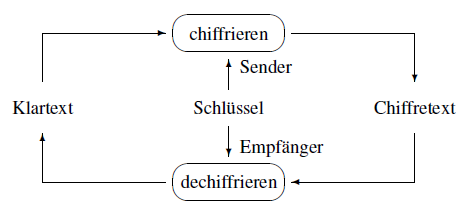
\includegraphics[width=\textwidth]{grafiken/verschluesselung.png}
    \caption[Kryptografische Verschlüsselung]{Kryptografische Verschlüsselung \\ Quelle: \cite[S. 1]{Watjen.2018}}
    \label{fig:verschluesselung}
\end{figure}

Wätjen beshreibt Kryptografische System, auch Kryptosystem genannt, als ein System aus fünf Komponenten:

\begin{itemize}
\item[ 1. ]  Klartextraum $M$
\item[ 2. ]  Chiffretextraum C
\item[ 3. ]  Schlüsselraum K
\item[ 4. ]  Familie von Chiffriertransformationen $E_k:M \rightarrow C$ mit $k \in K$
\item[ 5. ]  Familie von Dehiffriertransformationen $D_k:C \rightarrow M$ mit $k \in K$
\end{itemize}

Laut Watjen sind $M$, $C$ und $K$ höchstens, abzählbare Mengen. Eine Chiffriertransformation $E_K$ wird durch einen Schlüssel $K$ und einen Chiffrieralgorithmus $E$ definiert, welcher für jede Familie gleich ist. Eine Dechiffriertransformation $D_K$ wird ebenfalls durch einen Schhlüssel $K$ bestimmt. Desweiteren sollen die Kryptografischen Systeme nach Watjen die folgenden drei Eigenschaften aufweisen \cite[S. 3]{Watjen.2018}:

\begin{itemize}
\item[ (1) ]  Chiffrier- und Dechiffriertransformationen müssen für alle Schlüssel effizient berechnet werden können.
\item[ (2) ]  Kryptographische Systeme müssen leicht zu benutzen sein. Das bedeutet, dass es ohne Schwierigkeiten möglich sein muss, einen Schlüssel $K$ sowie die zugehörigen Abbildungen
$E_K$ und $D_K$ zu finden.
\item[ (3) ]  Die Sicherheit des Systems sollte auf der Geheimhaltung der Schlüssel und nicht
auf der Geheimhaltung der Algorithmen beruhen. Die Kenntnis der Methode des
Chiffrierens und Dechiffrierens soll also noch nicht den Klartext liefern.
\end{itemize}

Die heutzutage eingesetzten kryptographischen Systeme ermöglichen also eine schnelle und sichere Übertragung von sensiblen Informationen. Die Übertragung der Daten läuft also privat ab, da ein abgefangenes Chiffrat nicht direkt lesbar ist. Doch wie helfen dabei Primzahlen?\\

Primzahlen sind aufgrund ihrer hervorragenden Eigenschaften für die Kryptographie nützlich. Schon der Mathematiker Riemann suchte nach einer Ordnung hinter den Primzahlen. Die Verteilung der Primzahlen scheint pseudozufällig. Dadurch können nur sehr schwierig Vorhersagen zu kryptographischen Systemen getroffen werden, die Primzahlen verwenden.  Viele Verfahren, welche den Klartext in einen Chiffretext überführen, benötigen für ihren Algorithmus Primzahlen. Ein gutes Beispiel ist der Diffie-Hellmann-Schlüsselaustausch (DHKE). In  \ref{sec:DHKE} wird gezeigt, wie Primzahlen beim DHKE verwendet werden.

XXX




\section{Algebraische Strukturen}
Definiert durch die Zahlentheorie und als zentraler Untersuchungsgegenstand des mathematischen Teilgebietes der universellen Algebra, liefern algebraische Strukturen die Basis zur Realisierung komplexer symmetrischer und asymmetrischer Kryptosysteme, weshalb wir im folgenden Kapitel die Eigenschaften relevanter algebraischer Strukturen näher betrachten wollen. Darüber hinaus möchten wir Ihnen auch einige Werkzeuge zum Rechnen in der jeweiligen algebraischen Struktur an die Hand geben, welche zur späteren Realisierung von Kryptosystemen benötigt werden.\\

Unter einer sehr allgemeinen Betrachtung ist eine mathematische Struktur eine Liste nichtleerer Mengen, genannt Trägermengen, mit Elementen aus den Trägermengen, genannt Konstanten, und mengentheoretischer Konstruktionen über den Trägermengen. Diese sind konkret Funktionen über den Trägermengen. Im Weiteren beschränken wir uns auf den Fall einer einzigen Trägermenge, wodurch die Strukturen als homogen bezeichnet werden können.\cite[S. 355]{Berghammer.2021}

\paragraph{Definition: Homogene algebraische Struktur}
Eine homogene algebraische Struktur ist ein Tupel $(M,c_1,\dots,c_m,f_1,\dots,f_n)$ mit $m,n \in \mathbb{N}$ und $n \geq 1$. Dabei ist $M$ eine nichtleere Menge, genannt \textbf{Trägermenge}, alle $c_i$ sind Elemente aus $M$, genannt die \textbf{Konstanten}, und alle $f_i$ sind $s_i$-stellige Funktionen $f_i:M \rightarrow M$ im Fall $s = 1$ und $f_i:M^{s_i} \rightarrow M$ im Fall $s_i>1$, genannt die (inneren) \textbf{Operationen}. Die lineare Liste$(0,\dots,0,s_1,\dots,s_n)$ mit $m$ Nullen heißt \textbf{Typ} oder die \textbf{Signatur}.\newline

Laut dieser Definition muss eine homogen algebraische Struktur nicht unbedingt Konstanten enthalten, jedoch mindestens eine Operation. Das Paar $(\mathbb{N},+)$ bildet beispielsweise eine homogene algebraische Struktur des Typs (2). Das 5-Tupel $(\mathbb{N},0,1,+,\cdot)$ bildet ebenfalls eine homogen algebraische Struktur des Typs (0,0,2,2).

Algebraische Strukturen unterscheiden sich grundsätzlich durch ihren Typ. Wirklich charakterisiert werden sie aber erst durch die jeweils geltenden Axiome, d.h. bestimmte Eigenschaften, welche für die Konstanten und Operationen gefordert werden. Durch die Hinzunahme immer weiterer Axiome, entsteht eine Hierarchie immer feinerer Strukturen, an deren Anfang der Monoid steht.\cite[S. 355, 356]{Berghammer.2021}

\subsection{Monoid}

\paragraph{Definition: Monoid}
Eine algebraische Struktur $(M,e,\cdot)$ des Typs (0,2) heißt ein Monoid, falls für alle $x,y,z\in M$ die folgenden Monoid Axiome gelten:
\begin{itemize}
    \item (Ass) $x \circ (y \circ z) = (x \circ y) \circ z$
    \item (Neu) $e \circ x = x = x \circ e$
\end{itemize}  Gilt zusätzlich noch für alle $x,y \in M$ die Gleichung $x \circ y = y \circ x$, so heiß $(M,e,\circ)$ ein \textbf{kommutatives Monoid}.\\

Die erste und die letzte Gleichung bilden das Assoziativ- und Kommutativgesetz ab. Durch die mittlere Gleichung wird ein neutrales Element $e$ bezüglich der Operation gefordert, wobei sowohl die \textbf{Linksneutralität} als auch die \textbf{Rechtsneutralität} spezifiziert wird.\\

Einfache Beispiele für Monoide sind $(\mathbb{N},0,+)$, $(\mathbb{N},1,\cdot)$ und $(\mathbb{Z},0,+)$. Die Potenzierung in solchen Monoiden ist folgendermaßen definiert.\cite[S. 356]{Berghammer.2021}

\paragraph{Definition: Potenzierung}
In einem Monoid $(M,e,\cdot)$ definiert man die $n$-te \textbf{Potenz} $x^n$ von $x \in M$ durch $x^0 := e$ und $x^{x+1} = x \cdot x^n$ für alle $n \in \mathbb{N}$.\\

Daraus ergibt sich für den Monoid $(\mathbb{N},1,\cdot)$ die aus $\mathbb{R}$ gewohnte Potenzierung. Nach welcher für ein $x \in \mathbb{N}$ die Potenzierung $x^n = x_1 \cdot x_2 \cdot \dots \cdot x_n$ ergibt. Betrachtet man jedoch den Monoid $(\mathbb{N},0,+)$, so ergibt analog dazu für ein $x \in \mathbb{N}$ die Potenzierung $x^n = x_1 + x_2 + \dots + x_n = x \cdot n$, was also einer Multiplikation von $x$ mit $n$ entspricht \cite[S. 356, 357]{Berghammer.2021}.

\subsection{Gruppe}\label{sec:gruppe}

\paragraph{Definition: Gruppe}
Eine algebraische Struktur $(G,e,\circ,inv)$ des Typs $(0,2,1)$ heißt \textbf{Gruppe}, falls für alle $x,y,z \in G$ die folgenden Axiome gelten:

\begin{itemize}
    \item (Ass)    $x \circ (y \cdot z) = (x \circ y) \circ z$
    \item (Neu)    $e \circ x = x$
    \item (Inv)    $inv(x) \circ x = e$
\end{itemize}

Gilt wiederum die Gleichung $x \circ y = y \circ x$ für alle $x,y \in G$, so heißt $(G,e,\circ,inv)$ eine \textbf{kommutative Gruppe} oder Abelsche Gruppe. Die Gruppenoperation $\circ$ ist \textit{abgeschlossen}. D.h. für alle $a,b \in G$ gilt $a \circ b = c \in G$.

In jeder Gruppe $(G,e,\circ,inv)$ gelten für alle $x \in G$ folgende Formeln \cite[S. 357-359]{Berghammer.2021}:
\begin{align*}
&x \circ x = x \Rightarrow x = e
&&x \circ e = x
&&x \circ inv(x) = e
\end{align*}
Diese lassen sich durch Anwendung der obigen Axiome und ein wenig Logik beweisen. Die Beweise können im Buch von Berghammer unter \cite[S. 358, 359]{Berghammer.2021} nachvollzogen werden. Die folgenden Formeln beziehen sich auf die Eindeutigkeit neutraler und inverser Elemente in Gruppen.
\begin{align*}
&(\forall z \in G: x \circ z = z) \Rightarrow x = e
&&x \circ y = e \Rightarrow x = inv(y)
\end{align*}
Auch diese lassen sich mit den schon bekannten Gruppengesetzen beweisen, was unter \cite[S. 358, 359]{Berghammer.2021} nachgeschlagen werden kann. Weiterhin sind die folgenden Rechenregeln für Gruppen zu nennen.

\begin{align*}
&inv(x \circ y) = inv(x) \circ inv(y)
&&inv(inv(x)) = x
&&inv(e) = e
\end{align*}

Die erste Gleichung lässt sich leicht durch folgende Rechnung zeigen:
$$(inv(y) \circ inv(x)) \circ (x \circ y) = inv(y) \circ (inv(x) \circ x) \circ y = inv(y) \circ e \circ y = inv(y) \circ y = e$$
Damit ist gezeigt, dass $inv(y) \circ inv(x)$ linksinvers zu $x \circ y$ ist. Unter dieser Prämisse und der Eindeutigkeit der inversen Elemente muss die erste Gleichung gelten. Die beiden anderen Gleichungen lassen sich auf sehr ähnliche Weise zeigen.\\

Um Gruppen ein wenig anschaulicher zu machen, betrachten wir im Folgenden ein paar Beispiele:
\begin{itemize}
\item $(\mathbb{Z}, +)$ ist eine Gruppe. $\mathbb{Z} = \{\dots, -1, 0, 1, \dots \}$ ist die Menge der ganzen Zahlen, welche zusammen mit der Addition als Gruppenoperation eine abelsche Gruppe bildet, wobei $e = 0$ das neutrale Element und $-a$ das Inverse eines beliebigen Elements $a \in \mathbb{Z}$ ist.
\item Ein Gegenbeispiel ist $(\mathbb{Z} \setminus \{0\}, \cdot)$. Die Menge der ganzen Zahlen (ohne die 0) mit der Multiplikation als Gruppenoperation bildet keine Gruppe, da es kein Inverses Element $a^(-1)$ für jedes Element $a \in \mathbb{Z}$ gibt \cite[S. 239, 240]{Paar.2016}.
\end{itemize}
\subsection{Zyklische Gruppe} \label{sec:zyklische_Gruppe}
Die eben eingeführten Gruppen besitzen unendlich viele Elemente. Für die Kryptographie interessant sind jedoch endliche algebraische Strukturen, weshalb im Folgenden die endlichen Gruppen eingeführte werden.

\paragraph{Definition: Endliche Gruppe}
Eine Gruppe $(G, \circ)$ ist \textit{endlich}, wenn sie eine endliche Anzahl an Elementen hat. Die Anzahl der Elemente der Gruppe wird als 
\textit{Kardinalität} oder \textit{Ordnung} der Gruppe $G$ mit $|G|$ bezeichnet\cite[S. 241]{Paar.2016}.

Beispiele für endliche Gruppen sind:
\begin{itemize}
\item $(\mathbb{Z}_n, +):$ Die Kardinalität von $\mathbb{Z}_n$ ist $|\mathbb{Z}_n| = n$, da $\mathbb{Z}_n = \{0,1,2,\dots ,n-1\}$.
\item $(\mathbb{Z}^*_n, \cdot):$ Die Menge $\mathbb{Z}^*_n$ besteht aus den positiven Zahlen kleiner $n$, die teilerfremd zu $n$ sind, d.h. es gilt $ggt(a,n) = 1$ für jedes $a \in \mathbb{Z}^*_n$. Die Kardinalität ist daher durch die eulersche Phi-Funktion gegeben, d.h. $|\mathbb{Z}^*_n| = \Phi(n)$. So hat beispielsweise die Gruppe $\mathbb{Z}^*_9$ eine Kardinalität von $\Phi(9) = 3^2 - 3^1 = 6$. Die sechs Gruppenelemente sind ${1,2,4,5,7,8}$.
\end{itemize}

Für die Konstruktion eines DLPs wird eine weitere Spezialisierung der endlichen Gruppen benötigt, die sogenannten zyklischen Gruppen. Einleitend dazu wollen wir zunächst den Begriff der Ordnung eines Elements definieren.

\paragraph{Definition: Ordnung eines Elements}
Die \textit{Ordnung}  $ord(a)$ eines Elements $a$ einer Gruppe $(G, \circ)$ ist die kleinste positive ganze Zahl $k$ mit $$a^k = \underbrace{a \circ a \circ \dots \circ a}_{\text{$k$ mal}} = e$$ wobei $e$ neutrales Element von $G$ ist \cite[S. 241]{Paar.2016}.

Nachfolgend wollen wir ein Beispiel betrachten:

Wir suchen die Ordnung von $a=3$ in der Gruppe $\mathbb{Z}^*_{11}$. Dazu berechnen wir die Potenzen von $a$ bis wir das neutrale Element 1 erhalten.
\begin{align*}
&a^1 = 3 \\
&a^2 = a \cdot a = 9\\
&a^3 = a^2 \cdot a =  27 \equiv 5 \text{ mod } 11\\
&a^4 = a^3 \cdot a =  15 \equiv 4 \text{ mod } 11\\
&a^5 = a^4 \cdot a =  12 \equiv 1 \text{ mod } 11\\
\end{align*}
Aus der letzten Zeile folgt ord(3) $= 5$ in $\mathbb{Z}^*_{11}$.

Es ist interessant zu sehen, was passiert, wenn man weiter mit $a$ multipliziert:
\begin{align*}
&a^6 = a^5 \cdot a = 1 \cdot a \equiv 3 \text{ mod } 11\\
&a^7 = a^5 \cdot a^2 = 1 \cdot a^2 \equiv 9 \text{ mod } 11\\
&a^8 = a^5 \cdot a^3 = 1 \cdot a^3 \equiv 5 \text{ mod } 11\\
&a^9 = a^5 \cdot a^4 = 1 \cdot a^4 \equiv 4 \text{ mod } 11\\
&a^{10} = a^5 \cdot a^5 = 1 \cdot a^5 \equiv 1 \text{ mod } 11\\
&a^{11} = a^{10} \cdot a = 1 \cdot a \equiv 3 \text{ mod } 11\\
&\qquad \vdots
\end{align*}
Wie zu sehen ist, durchlaufen die Potenzen von $a$ nach Erreichen des neutralen Elements $e$ immer wieder die Sequenz $\{3,9,5,4,1\}$. Mit diesem Wissen können wir jetzt eine zyklische Gruppe definieren \cite[S. 241, 242]{Paar.2016}.

\paragraph{Definition: Zyklische Gruppe}
Eine Gruppe $G$, die ein Element $\alpha$ mit der maximalen Ordnung ord($\alpha$) $= |G|$ enthält nennt man \textit{zyklisch}. Elemente mit maximaler Ordnung nennt man \textit{primitive Elemente} oder \textit{Generatoren} \cite[S. 242]{Paar.2016}.\\

Der Name \textit{Generator} kommt daher, dass durch die Potenzierung $\alpha^i = a$ des primitiven Elements jedes andere Gruppenelement $a$ dargestellt werden kann, also die gesamte Gruppe \textit{generiert} wird. Das folgende Beispiel zeigt die Erzeugung der zyklischen Gruppe $\mathbb{Z}^*_{11}$ durch das primitive Element $\alpha = 2$.
\begin{align*}
&a = 2 \qquad \qquad \qquad a^6 \equiv 9 \text{ mod } 11\\
&a^2 = 4 \qquad \qquad \qquad a^7 \equiv 7 \text{ mod } 11\\
&a^3 = 8 \qquad \qquad \qquad a^8 \equiv 3 \text{ mod } 11\\
&a^4 \equiv 5 \text{ mod } 11 \qquad a^9 \equiv 6 \text{ mod } 11\\
&a^5 \equiv 10 \text{ mod } 11 \qquad a^{10} \equiv 1 \text{ mod } 11\\
\end{align*}

Aus der letzten Gleichung folgt, dass ord$(a=2)=10=|\mathbb{Z}^*_{11}|$. Damit ist gezeigt, dass das Element $a = 2$ wirklich ein Generator der zyklischen Gruppe $\mathbb{Z}^*_{11}$ ist.

Wie man aus den eben gezeigten Beispielen erkennen kann, sind einige Gruppenelemente Generatoren der Gruppe und andere nicht. Welche Ordnungen der Elemente in einer zyklischen Gruppe vorkommen hängt davon ab, welche natürlichen Zahlen die Gruppenkardinalität teilen. Betrachten wir nun wieder die Gruppe $\mathbb{Z}^*_{11}$, deren Kardinalität $|\mathbb{Z}^*_{11}| = 10$ ist, so ergeben sich mögliche Ordnungen der Elemente von $1,2,5 \text{ und }10$, da diese die einzigen natürlichen Zahlen sind die $10$ teilen. Folgende Veranschaulichung zeigt dies \cite[S. 243, 244]{Paar.2016}.
\begin{align*}
&\text{ord }(1) = 1 \qquad \text{ord }(6) = 10\\
&\text{ord }(2) = 10 \qquad \text{ord }(7) = 10\\
&\text{ord }(3) = 5 \qquad \text{ord }(8) = 10\\
&\text{ord }(4) = 5 \qquad \text{ord }(9) = 5\\
&\text{ord }(5) = 5 \qquad \text{ord }(10) = 2\\
\end{align*}

\paragraph{Satz: Primitive Elemente in einer zyklischen Gruppe $G$}
Ist $G$ eine zyklische Gruppe, dann gilt:
\begin{enumerate}
\item Die Anzahl der primitiven Elemente in $G$ ist $\Phi (|G|)$.
\item Ist $|G|$ prim, dann sind alle Elemente $a \neq 1 \in G$ primitiv \cite[S. 244]{Paar.2016}.
\end{enumerate}

Die erste Eigenschaft kann leicht gezeigt werden durch, $\Phi(10) = (5-1)(2-1) = 4$. Es muss also vier primitive Elemente in $\mathbb{Z}^*_{11}$ geben, welche konkret die Elemente $2,6,7$ und $8$ sind. Die zweite Eigenschaft folgt implizit aus der ersten, da bei einer primen Kardinalität der Gruppe keine natürliche Zahl außer der $1$ und der Kardinalität selber die Gruppenkardinalität teilt, und diese somit die einzigen möglichen Elementordnungen sind. Da nur das Element $1$ die Ordnung $1$ haben kann, haben alle anderen Elemente die Ordnung $|G|$, sind also Generatoren der Gruppe \cite[S. 244]{Paar.2016}.

\subsection{Untergruppen} \label{sec:untergruppen}
Untermengen innerhalb zyklischer Gruppe können wiederum selbst Gruppen sein. Solche werden als Untergruppen bezeichnet. Im Fall von zyklischen Gruppen ist die Anzahl der jeweiligen Untergruppen leicht zu ermitteln. Sie entspricht nämlich genau der Anzahl an natürlichen Teilern der Gruppenkardinalität, wie aus dem folgenden Satz von Lagrange hervorgeht.

\paragraph{Satz: Satz von Lagrange}
Sei $H$ eine Untegruppe von $G$. Dann teilt $|H|$ die Gruppenkardinalität $|G|$ \cite[S. 245]{Paar.2016}.

Das \textit{Finden} zyklischer Untergruppen innerhalb einer zyklischen Gruppe wird durch folgenden Satz gezeigt.

\paragraph{Satz: zyklische Untergruppen}
Sei $(G, \circ)$ eine zyklische Gruppe. Dann ist jedes Element $a \in G$ mit ord$(a) = s$ ein primitives Element einer zyklischen Untergruppe mit $s$ Elementen \cite[S. 244]{Paar.2016}.\\

Die Kernaussage dieses Satzes ist, dass jedes Element einer zyklischen Gruppe Generator einer zyklischen Untergruppe ist.  Wir betrachten erneut die zyklische Gruppe $\mathbb{Z}^*_{11}$. Wie oben bereits gezeigt hat das Gruppenelement $a=3$ die Ordnung $5$, ist also Generator einer Untergruppe mit mit $5$ Elementen. Die Elemente dieser Untergruppe sind eben jene, welche durch die Potenzierung von $3$ mod $11$ erzeugt werden können, also $\{3,9,5,4,1\}$. So kann für jedes Element verfahren werden, alle Untergruppen von $\mathbb{Z}^*_{11}$ gezeigt werden können. Folgende Aufstellung zeigt beispielhaft alle Untergruppen von $\mathbb{Z}^*_{11}$.
\begin{align*}
&\text{Ordnung: } 1 \text{ Generatoren: } \{1\} \text{ Elemente: }\{1\}\\
&\text{Ordnung: } 2 \text{ Generatoren: } \{10\} \text{ Elemente: }\{1,10\}\\
&\text{Ordnung: } 5 \text{ Generatoren: } \{3,4,5,9\} \text{ Elemente: }\{1,3,4,5,9\}\\
&\text{Ordnung: } 10 \text{ Generatoren: } \{2,5,7,8\} \text{ Elemente: } \{1,2,3,4,5,6,7,8,9,10\}\\
\end{align*}
Wie zu erkennen ist, kann es mehrere Generatoren der selben Untergruppe geben. Außerdem interessant ist die Tatsache, dass Untergruppen primer Ordnung $p$ abgesehen von dem neutralen $1$ keine Überschneidungen mit anderen Untergruppen primer Ordnung aufweisen, da jedes Element die Ordnung $p$ hat und somit Generator der Untergruppe ist. Dies verdeutlicht, dass der Satz \textit{Primitive Elemente in einer zyklischen Gruppe} auch für zyklische Untergruppen gilt \cite[S. 244-246]{Paar.2016}.

Der folgende Satz fasst die Erkenntnisse des letzten Abschnitts zusammen und gibt eine Methode zur Konstruktion einer Untergruppe für eine gegebene zyklische Gruppe.

\paragraph{Satz: Konstruktion einer zyklischen Untergruppe}
Sei $G$ eine endliche zyklische Gruppe der Ordnung $n$ und sei $\alpha$ ein Generator von $G$. Dann existiert für jede ganze Zahl $k$, die $n$ teilt, genau eine zyklische Untergruppe $H$ von $G$ mit der Ordnung $k$. Diese Untergruppe wird erzeugt von $\alpha^{n/k}$. $H$ besteht genau aus den Elementen $a \in G$, die die Bedingung $a^k = 1$ erfüllen. Es gibt keine weiteren Untergruppen \cite[S. 246]{Paar.2016}.\\

Mit anderen Worten sagt dieser Satz, dass lediglich ein primitives Element $\alpha$ und die Ordnung einer zyklischen Gruppe $|G|$ benötigt wird, um alle Untergruppen von $G$ zu konstruieren. Im folgenden Beispiel wollen wir dies zu Konstruktion einer Untergruppe anwenden.\\

Betrachten wir dazu erneut die zyklische Gruppe $\mathbb{Z}^*_{11}$ und das primitive Element $\alpha = 6$. Wenn wir nun eine Generator $\beta$ der Untergruppe mit der Ordnung $k = 5$ finden möchten, berechnen wir:
$$\beta = \alpha^{n/k} = 6^{10/5} = 6^2 = 36 \equiv 3 \text{ mod } 11$$
Wie wir oben schon gezeigt haben ist $3$ tatsächlich ein Generator der Untergruppe $\{1,3,4,5,9\}$ mit $k = 5$ Elementen\cite[S. 246]{Paar.2016}.

\subsection{Ring}
Ein \textbf{Ring} ist eine algebraische Struktur $(R,0,1,+,\cdot,-)$ des Typs $(0,0,2,2,1)$ mit den folgenden Eigenschaften:
\begin{enumerate}
\item Es ist $(R,0,+,-)$ eine kommutative Gruppe
\item Es ist $(R,1,\cdot)$ ein Monoid.
\item Für alle $x,y,z \in R$ gelten die Distributivgesetze $x(y+z) = xy$ und $(y+z)x = yx +zx$
\end{enumerate}
Ist $(R,1,\cdot)$ ein kommutatives Monoid, so nennt man $(R,0,1,+,\cdot,-)$ einen kommutativen Ring.

\subsection{Körper} \label{sec:koerper}
Ein Körper ist eine spezielle Form des Rings. Die Definition des Körpers wurde aus \cite[S. 364-365]{Berghammer.2021} entnommen. Ein Ring $(K,0,1,+,\cdot,-)$ heißt \textbf{Körper}, wenn er kommutativ ist sowie gilt, dass $0 \neq 1$. Weiterhin muss folgende Formel $$x \neq 0 \Rightarrow \exists y \in K : yx = 1$$ für alle $x \in K$ gelten.\\

Berghammer beschreibt in seinem Buch ein Stilbruch bei der Definition der Körper. Im Vergleich zu den Monoiden, Gruppen und Ringen erfordert der Körper eine Ungleichung als Axiom. Weiterhin existiert ein noch komplizierteres Axiom, nämlich eine Implikation mit einer Ungleichung als linker und einer Existenzquantifizierung als rechter Seite. Weiterhin ist im Gegensatz zu den Gruppen das linksinverse Element y zu x im zweiten Axiom bezüglich der Multiplikation nicht durch eine Spezifikation, sondern durch eine Existenzquantifizierung spezifiziert. Dadurch spezifiziert Berghammer Körper als algebraische Strukturen, welche nicht gleichungsdefiniert sind \cite[S. 364-365]{Berghammer.2021} Der Satz $x \neq 0$ impliziert, dass es nur ein linksinverses Element geben kann. Aufgrund der Kommutativität von \glqq$\cdot$\grqq{} ist dieses linksinverse Element auch rechtsinvers.\\

Desweiteren haben Körper weitere Eigenschaften. Diese sind dem Buch über elementare Algebra und Zahlentheorie von Stroth und Waldecker entnommen \cite[S. 57-59]{Stroth.2019}.Sei $K$ ein Körper. Dann gilt
\begin{enumerate}
\item Die kleinste natürliche Zahl $n$ mit der Eigenschaft $\underbrace{1_{K} + ... + 1_{K} = 0_{K}}_{\substack{n-mal}}$ wird die \textbf{Charakteristik} von $K$ genannt. Mann schreibt das als char($K$)$ = n$. Gibt es keine solche Zahl n, so schreibt man char($K$)$ = 0$. 
\item Ein Teilkörper von $K$ ist ein Teilring, der mit Einschränkung der Verknüpfungen selbst ein Körper ist.
\item Der Durchschnitt aller Teilkörper von $K$ heißt  \textbf{Primkörper} von $K$.
\item Zwei Körper heißen  \textbf{isomorph} genau dann, wenn es einen bijektiven Ringhomomorphismus von dem einen in den anderen gibt.
\end{enumerate}

Wie man sieht, ist ein Körper ein sehr komplexes Gebilde. Einige bekannte Körper sind die Mengen $\mathbb{Q}$, $\mathbb{R}$ und $\mathbb{C}$ mit der Multiplikation und der Addition innerhalb der Körper. Unter den Körpern befinden sich auch die endlichen Körper. Endliche Körper hat eine besondere Eigenschaft. Diese bezieht sich auf die Endlichkeit und der Anzahl ihrer Elemente. Die folgenden Definitionen und Aussagen sind dem Script zur Kryptografie von Reinhold Hübl entnommen  \cite[S. 266]{Dr.ReinholdHubl.2022}.\\

\paragraph{Definition: Endliche Körper und Primkörper}
Sei $K$ ein Körper $(K,+,\cdot)$. $K$ ist ein endlicher Körper, wenn $\lvert K \rvert < \infty$. Ist $p$ eine Primzahl, so schreibt man $\mathbb{F}_p$ für den Körper $\mathbb{Z}/p\mathbb{Z}$. Für eine Primzahl $p$ heißt der Körper $\mathbb{F}_p$ \textbf{Primkörper} der Charakteristik $p$. Dabei wird $\mathbb{F}_p$ durch folgende Elemente beschrieben: $$\mathbb{F}_p =  \{1, ..., p - 1\}$$ Alle Elemente in $\mathbb{F}_p$ sind teilerfremd zu $p$. Daher sind alle Äquivalenzklassen $$[1], [2], ..., [p - 1]$$ Einheiten in $\mathbb{F}_p$. Durch $x \in \mathbb{F}_p \backslash \{0\}$ hat damit jedes Element ein Inverses. Damit wurde eine weitere wichtige Eigenschaft von Körpern gefunden, nämlich dass jedes Element in diesem Körper außer der Zahl Null ein Inverses in Bezug auf die Multiplikation hat. Der folgende Satz wurde aus dem Script von Hübl entnommen. Es handelt sich um einen Satz von Fermat \cite[S. 269]{Dr.ReinholdHubl.2022}.

\paragraph{Satz:}
Die Einheitengruppe $\mathbb{F}_p^*$ eines endlichen Körpers $\mathbb{F}_p$ ist zyklisch.\\

Im Kapitel \ref{sec:gruppe} wurde das Inverse definiet. Für die Rechnungen in einem endlichem Körper $\mathbb{F}_p$ können keine rationale Zahlen $\mathbb{Q}$ dargestellt werden. In manchen Rechnungen kommt man jedoch nicht darum, mit Brüchen oder etwaigen rationalen Zahlen zu hantieren. Damit man jedoch eindeutige Ergebnisse in $\mathbb{F}_p$ bekommt, muss man den Kehrwert über das Inverse bilden. Nimmt man als Beispiel die Zahl $\frac{3}{11}$ in $\mathbb{F}_{17}$. Da es keine rationalen Zahlen in der zyklischen Gruppe gibt, muss man anders an die Werte kommen. Als erstes schreibt man um: $\frac{3}{11} = 3 \cdot \frac{1}{11}$. Jetzt berechnet man das inverse Element von 11 in $\mathbb{F}_{17}$. Das inverse Element ist die Zahl 14, da $11 \cdot 14 \equiv 1 \text{ mod } 17$. Man rechnet $\frac{3}{11} = 3 \cdot \frac{1}{11} = 3 \cdot 14 = 42 \equiv 8 \text{ mod } 17$.\\ 

Das Inverse berechnet man üblicherweise mit dem erweiterten euklidischen Algorithmus oder Potenzregeln mit Zuhilfenahme des kleinen Satzes von Fermat. Für diese Studienarbeit wird jedoch der erweiterte euklidische Algorithmus betrachtet. Mit diesem kann man das multiplikative Inverse der Zahl $a^{-1}$ der Zahl $a \neq 0$ bestimmen, also den Kehrwert von $a$. Um den erweiterten euklidischen Algorithmus durchzuführen, muss im Vorfeld der reguläre euklidische Algorithmus durchgeführt worden sein. Der euklidische Algorithmus berechnet den größten gemeinsamen Teiler von zwei Zahlen $a$ und $b$. In einer Internetveröffentlichung der Hochschule für Technik in Stuttgart wird die Grundfunktionsweise des euklidischen Algorithmus in einem Satz auf den Punkt gebracht: \textit{Teilen so lange mit Rest, bis der Rest 0 erreicht} \cite[S. 2]{HFT.Stuttgart}. Bei dem Iterationsschritt vor dem Schritt, bei welchem die 0 erreicht wurde, ist der Rest der $ggt(a, b)$.\\

Als erstes legt man zwei Zahlen $a$ und $b$ fest, für welche der euklidische Algorithmus durchgeführt werden soll. Im ersten Schritt teilt man die kleinere Zahl durch die größere und schreibt den Rest auf. Im nächsten Schritt teilt man die kleinere Zahl durch den Rest und schreibt dann wieder den Rest auf. Dies wird solange wiederholt, bis die 0 erreicht ist. Die Vorgehensweise soll anhand von zwei Beispielen erfolgen. Als erstes Beispiel wird $a = 174$ und $b = 102$ gesetzt.
\begin{align*}
&174 = 1 \cdot 102 + 72\\
&102 = 1 \cdot 72 + 30\\
&72 = 2 \cdot 30 + 12\\
&30 = 2 \cdot 12 + 6\\
&12 = 2 \cdot 6 + 0
\end{align*}
Als erstes haben wir eine Gleichung aufgestellt. Die Zahl 174 setzt sich aus $1 \cdot 102$ und dem Rest 72 zusammen. Im nächsten Schritt nimmt man die größte Zahl und stellt sie links von der Gleichung, in diesem Fall die Zahl 102. Man prüft, wie oft der vorherige Rest 72 in die 102 reinpasst. Der Rest ist die Zahl 30. Die Zahl 102 wird nun durch 72 substituiert. Der vorherige Rest 30 passt zwei mal in die 72. Der Rest ist 12. Die 30 wird im nächsten Iterationsschritt links der Gleichung gesetzt.  Der vorherige Rest 12 passt zwei mal in die Zahl 30 rein und es ergibt sich ein Rest von 6. Im nächsten Iterationsschritt setzen wir die 12 links in die Gleichung ein. Der vorherige Rest 6 passt genau zwie mal in die 12 rein. Da sich keiN Rest ergibt, ist der Algorithmus vollständig durchgelaufen. Im vorletzten Iterationsschritt kann man den größten gemeinsamen Teiler ablesen. Der durchgeführte euklidische Algorithmus ergibt, dass der $ggt(174, 102)$ die Zahl 6 ist.\\

Hübl beschreibt den euklidischen Algorithmus in seinem Script über eine allgemeine Formel \cite[S. 256-257]{Dr.ReinholdHubl.2022}. Gegeben sei $a$ und $b$ mit $b \geq a$. Sei $i = 0$, $r_{1} = a$ und $r_{0} = b$. Man dividiert $r_{i}$ durch $r_{i + 1}$ mit Rest durch folgende Formel: $$r_{i} = q \cdot r_{i + 1} + c$$
Dabei ist q eine natürliche Zahl und der Rest $c \in \{0, 1, ..., r_{i + 1} - 1\}$. Falls $b = 0$, dann ist der Algorithmus fertig. Falls $b \neq 0$, setzt man $r_{i + 2} = c$ und $i = i + 1$. Dies wird so oft wiederholt, bis der Rest 0 ist und der Algorithmus durchgelaufen ist. Der größte gemeinsame Teiler ist in beiden Fällen der Rest im vorletzten Iterationsschritt vor dem Erreichen der 0.\\

Nun wird ein etwas längeres Beispiel betrachtet. Man setzt $a = 575$ und $b = 839$. Dadurch ist  $i = 0$, $r_{0} = a = 839$ und $r_{1} = b = 575$.
\begin{align*}
&i = 0: \qquad 839 = 1 \cdot 575 + 264\text{. Man setzt } r_{2} = 264\\
&i = 1: \qquad 575 = 2 \cdot 264 + 47\text{. Man setzt } r_{2} = 47\\
&i = 2: \qquad 264 = 5 \cdot 47 + 29\text{. Man setzt } r_{2} = 29\\
&i = 3: \qquad 47 = 1 \cdot 29 + 18\text{. Man setzt } r_{2} = 18\\
&i = 4: \qquad 29 = 1 \cdot 18 + 11\text{. Man setzt } r_{2} = 11\\
&i = 5: \qquad 18 = 1 \cdot 11 + 7\text{. Man setzt } r_{2} = 7\\
&i = 6: \qquad 11 = 1 \cdot 7 + 4\text{. Man setzt } r_{2} = 4\\
&i = 7: \qquad 7 = 1 \cdot 4 + 3\text{. Man setzt } r_{2} = 3\\
&i = 8: \qquad 4 = 1 \cdot 3 + 1\text{. Man setzt } r_{2} = 1\\
&i = 9: \qquad 3 = 3 \cdot 1 + 0\text{.}\longrightarrow\text{\textbf{STOPP}}
\end{align*}
Die durchgeführte Rechnung ergibt, dass der $ggt(839, 575)$ die Zahl 1 ist.\\


Der euklidische Algorithmus liefert nur den größten gemeinsamen Teiler und nicht das Inverse. Um das Inverse zu erlangen, muss der euklidische Algorithmus zurückgerechnet werden. Diese Rückrechnung wird auch als der erweiterte euklidische Algorithmus bezeichnet. Dabei steht der Rest auf der linken Seite der Gleichung und man rechnet den euklidischen Algorithmus zurück, damit eine Gleichung der folgenden Form entsteht: $g = x \cdot a + y \cdot b$, wobei $a, b \in \mathbb{N} \ \{0\}$ und $ggt(a, b) = g$ \cite[S. 257]{Dr.ReinholdHubl.2022}. Folgend nun die Rückwärtsrechnung für das erste Beispiel.
\begin{align*}
&6 = 30 - 2 \cdot 12\\
&\enspace = 30 - 2 \cdot (72 - 2 \cdot 30) = 5 \cdot 30 - 2 \cdot 72\\
&\enspace = 5 \cdot (102 - 72) - 2 \cdot 72 = 5 \cdot 102 - 7 \cdot 72\\
&\enspace = 5 \cdot 102 - 7 \cdot (174 - 102) = 12 \cdot 102 -7 \cdot 174
\end{align*}
Damit wurde die Gleichung, die den Rest beschreibt gefunden. Diese ist $$6 = 12 \cdot 102 -7 \cdot 174$$ Diese kleine Beispielrechnung für den erweiterten euklidischen Algorithmus dient lediglich der Veranschaulichung der Funktionsweise. Da der Rest 6 ist hat 174 kein multiplikatives Inverses Modulo 102. Nun wird der erweiterte euklidische Algorithmus für das zweite Beispie angewendet, in welchem der Rest 1 ist und somit ein multiplikatives Inverses von 575 Modulo 839 existiert.
\begin{align*}
&1 = 4 - 3\\
&\enspace = 4 - (7 - 4)\\
&\enspace = 2 \cdot (11 - 7) - 7 = 2 \cdot 11 - 3 \cdot 7\\
&\enspace = 2 \cdot 11 - 3 \cdot (18 - 11) = 5 \cdot 11 - 3 \cdot 18\\
&\enspace = 5 \cdot (29 - 18) - 3 \cdot 18 = 5 \cdot 29 - 8 \cdot 18\\
&\enspace = 5 \cdot 23 - 8 \cdot (47 - 29) = 13 \cdot 29 - 8 \cdot 47\\
&\enspace = 13 \cdot (264 - 5 \cdot 47) - 8 \cdot 47 = 13 \cdot 264 - 73 \cdot 47\\
&\enspace = 13 \cdot 264 - 73 \cdot (575 - 2 \cdot 264) = 159 \cdot 264 - 73 \cdot 575\\
&\enspace = 159 \cdot (839 - 575) - 73 \cdot 575 = 159 \cdot 839 - 232 \cdot 575\\
\end{align*}
Damit wurde die Gleichung, die den Rest beschreibt gefunden. Diese ist $$1 = 159 \cdot 839 - 232 \cdot 575$$ Das Inverse wird nun wie folgt gefunden:
\begin{align*}
&1 \equiv x \cdot 575\text{ mod }839\\
&x \equiv \frac{1}{575}\text{ mod }839\\
&x = - 232 \equiv 607\text{ mod }839
\end{align*}
Das multiplikative Inverse von 575 Modulo 839 ist 607.\\

Bei der Berechnung der Punkte einer elliptischen Kurve wird oft das Inverse benötigt, da man durch die Formeln zur Berechnung der x-Werte und der y-Werte oft rationale Zahlen in Form von Brüchen bekommt. Durch das multiplikative Inverse kann eine rationale Zahl $\mathbb{Q}$ durch eine ganze Zahl $\mathbb{Z}$ dargestellt werden. Dies ist essentiell für die Rechnung in $\mathbb{F}_p$, da man nur mit ganzen Zahlen rechnet. Da die Rechnung von Hand sehr umständlich und unübersichtlich ist empfiehlt es sich, den euklidischen Algorithmus und den erweiterten euklidischen Algorithmus als Programm abzubilden. In Kapitel \ref{sec:python_euklid} wurde die beiden Algorithmen in Python umgesetzt.

\section{Allgemeines zur Verschlüsselung}
XXX

\subsection{Symmetrische und Asymmetrische Verschlüsselung}
XXX

\section{Das diskreter Logarithmusproblem} \label{sec:Das_diskrete_Logarithmusproblem}
Das DLP bildet die mathematische Grundlage für viele asymmetrische Kryptosysteme, wie den DHKE oder die Elgamal-Verschlüsselung. Etwas legere ausgedrückt könnte man das DLP als Baukasten für asymmetrische Kryptosysteme betrachten, da es für zyklische Gruppen verallgemeinert werden kann. Im Folgenden wollen wir zunächst das DLP in Primzahlkörpern betrachten. Hierzu greifen wir auf die in Kapitel \ref{sec:zyklische_Gruppe} erläuterten Eigenschaften zyklischer Gruppen zurück. 

\paragraph{Definition: Diskretes Logarithmusproblem (DLP) in $\mathbb{Z}^*_p$}
Gegeben sind die endliche zyklische Gruppe $\mathbb{Z}^*_p$ der Ordnung $p-1$, ein primitives Element $\alpha \in \mathbb{Z}^*_p$ und ein weiteres Element $\beta \in \mathbb{Z}^*_p$. Das DLP ist das Problem, eine ganze Zahl x im Bereich $1 \leq x \leq p-1$ zu finden, sodass: $$\alpha^x \equiv \beta \text{ mod } p$$\\

Wie in Kapitel XY gezeigt, muss ein solches $x$ existieren, da $\alpha$ ein primitives Element ist, was bedeutet dass jedes andere Gruppenelement durch die Potenzierung $\alpha^x$ dargestellt werden kann. Das gesuchte $x$ wird als \textit{diskreter Logarithmus} von $\beta$ zur Basis $\alpha$ bezeichnet. Formal beschrieben als: $$x = \text{ log}_\alpha \beta \text{ mod } p \text{.}$$

Anders als der gewöhnliche Logarithmus in $\mathbb{R}$ ist der diskrete Logarithmus in einer endlichen zyklischen Gruppe nicht effizient zu berechnen. Grund dafür sind die Eigenschaften endlicher zyklischer Gruppen. Denn wie in Kapitel XY gezeigt, generiert die Potenzierung eines primitiven Elements $\alpha$ die jeweilige zyklische Gruppe bzw. Untergruppe in einer nicht absehbaren Reihenfolge.\\

Für kleinere Gruppen lässt sich $x$ natürlich durch stumpfes Ausprobieren sog. \textit{brute Force} in einer kurzen Zeit ermitteln. Diskrete Logarithmen in ausreichend großen Gruppen sind jedoch sehr schwer zu ermitteln.\\

Um den diskreten Logarithmus $x$ von $\alpha^x \equiv \beta \text{ mod } p$ zu ermitteln muss ein potenzieller Angreifer jedes $x$ zwischen $1$ und $p-1$ als möglichen Exponenten ausprobieren. Der Erzeuger kann zum effizienten berechnen von $\beta$, jedoch den Square-and-Multiply-Algorithmus verwenden, was das DLP zu einer Einwegfunktion macht.\\

Neben dem trivialen brute Force Angriff auf das DLP gibt es weitere Verfahren, welche die Menge an möglichen $x$ Werten einschränken. Der Babystep-Giantstep-Algorithmus reduziert die Komplexität des DLPs von $O(n)$ auf $O(\sqrt{n})$. Noch weiter kann die Komplexität durch den Pohling-Hellman-Algorithums eingeschränkt werden. Durch diesen Angriff kann bei bekannter Primfaktorzerlegung der Gruppenordnung $n$, die Komplexität des DLPs auf $O(\sqrt{q})$ reduzieren, wobei $q$ der größte Faktor von $n$ ist. Aus diesem Grund wählt man in der Praxis eine Gruppe mit primer Ordnung für das DLP. Da die Ordnung von Gruppen $\mathbb{Z}^*_p$ dem Wert $p-1$ entspricht, der offensichtlich nicht prim ist, greift man auf Untergruppen von $\mathbb{Z}^*_p$ mit primer Ordnung zurück.\cite{Paar.2016}

\subsubsection{Das verallgemeinerte diskrete Logarithmusproblem}
Wie oben bereits erwähnt kann das DLP in jeglichen zyklischen Gruppen definiert werden. Bis jetzt haben wir immer die zyklische Gruppe $\mathbb{Z}^*_p$ betrachtet. Das DLP kann folgendermaßen verallgemeinert werden:

\paragraph{Definition: Verallgemeinertes diskretes Logarithmusproblem}
Gegeben sei eine endliche zyklische Gruppe $G$ mit der Gruppenoperation $\circ$ und der Kardinalität $n$. Wir betrachten ein primitives Element $\alpha \in G$ und ein weiteres Element $\beta \in G$. Das diskrete Logarihtmusproblem liegt darin, eine ganze Zahl $x$ im Bereich $1 \leq x \leq n$ zu finden, sodass:
$$\beta = \underbrace{\alpha \circ \alpha \circ \dots \circ \alpha}_{\text{$x$ mal}} = \alpha^x$$\\

Auch hier ist die Existenz von $x$ sicher, da $\alpha$ als primitives Element die gesamte Gruppe generiert. Das DLP lässt sich zwar in jeglichen zyklischen Gruppen definieren, jedoch ist es in einigen nicht \textit{schwierig} zu lösen, wodurch es keine Einwegfunktion mehr darstellt. Ein Beispiel dafür sind additive Gruppen $G = (\mathbb{Z}_p, +)$. Die $x$-fache Anwendung der Gruppenoperation auf einen Generator $\alpha$ zur Erzeugung eines Elements $\beta$ kann als \textit{Multiplikation} mod $p$ dargestellt werden. Der gesuchte Faktor $x$ lässt sich dann leicht durch die Multiplikation von $\beta$ und inv$(\alpha)$ berechnen. Letzteres lässt sich effizient mittels des EEAs ermitteln.

Gruppen auf denen ein DLP für kryptografische Zwecke definiert werden kann sind:
\begin{enumerate}
\item Multiplikative Gruppen des Primkörpers $\mathbb{Z}_p$ oder Untergruppen davon. Der DHKE nutz klassischerweise diese Gruppen. Auch die Elgamal-Verschlüsselung und der digitale Signaturalgorithmus (DSA) nutzen diese Gruppen.

\item Zyklische Gruppen welche über elliptischen Kurven gebildet werden. Das DLP ist in diesen Gruppen besonders schwer zu lösen, da kein Algorithmus bekannt ist, der die Komplexität des DLPs stark reduziert, wie dies beispielsweise beim DLP in $\mathbb{Z}^*_p$ durch den Babystep-Giantstep-Algorithmus möglich ist. Deshalb werden diese Gruppen in modernen Kryptosystemen zunehmend eingesetzt, mit dem Effekt, dass gleiche Sicherheit mit deutlich geringerer Schlüssellänge erzielt werden kann.

\item Multiplikative Gruppen von endlichen Körpern $GF(2^m)$ oder Untergruppen davon. Sie sind in der Praxis weniger verbreitet, und es nicht vollständig geklärt ob Angriffe auf das DLP in $GF(2^m)$ nicht effizienter sind als jene gegen das DLP in Primkörpern.

\item Hyperelliptische Kurven oder algebraische Varietäten, die auch Verallgemeinerungen von elliptischen Kurven sind. Trotz einiger Vorteile gegenüber den klassischen elliptischen Kurven, sind die hyperelliptischen Kurven in der Praxis nicht sehr verbreitet.
\end{enumerate}

Es gab im Laufe der Zeit einige weitere Vorschläge für mögliche Gruppen gegeben, welche jedoch nicht weiter verfolgt wurden, da sich meist herausstellte, dass das DLP einfacher zu lösen ist.\cite{Paar.2016}

\subsection{Diffie-Hellmann Key Exchange (DHKE)} \label{sec:DHKE}
Der DHKE wurde im Jahr 1976 von Whitfield Diffie und Martin Hellmann veröffentlicht. Damit ist er das älteste asymmetrsiche Verfahren überhaupt. Der DHKE bringt eine Lösung für das große Problem der symmetrischen Kryptografie: den Schlüsselaustausch. Er ermöglicht zwei Parteien den Austausch bzw. die Vereinbarung eines gemeinsamen Geheimnisses über einen unsicheren Kanal. Dabei nutzt der DHKE das im vorigen Kapitel \ref{sec:Das_diskrete_Logarithmusproblem} erläuterte DLP.  Prinzipiell beruht der DHKE auf der Idee, dass das Potenzieren in $\mathbb{Z}^*_p$ mit primen $p$ eine Einwegfunktion ist und die Exponentation kommutativ ist, d.h. $$k = (\alpha ^x)^y \equiv (\alpha ^y)^x \text{ mod } p.$$
Im Folgenden wird der der DHKE in seiner Grundform erläutert. In der Praxis wird der DHKE oft in erweiterter Form verwendet um Angriffen entgegenzuwirken.

Das Ziel der Kommunikationspartner Alice und Bob ist es einen gemeinsamen geheimen Schlüssel über einen unsicheren Kanal zu vereinbaren. Unter Umständen gibt es auch eine dritte Partei, welche die öffentlichen Parameter für den Schlüsselaustausch festlegt, dies kann aber auch durch Alice und Bob selbst ausgehandelt werden. Der DHKE besteht genau genommen aus zwei Protokollen: dem Set-up-Protokoll und dem Hauptprotokoll, das den eigentlichen Schlüsselaustausch durchführt. Das Setup sieht folgendermaßen aus:
\paragraph{Diffie-Hellman-Set-up:}
\begin{enumerate}
\item Wähle eine große Primzahl $p$
\item Wähle eine ganze Zahl $\alpha \in \{2,3,..., p-2\}$
\item Veröffentliche $p$ und $\alpha$
\end{enumerate}

Dies sind die öffentlichen Parameter manchmal auch als \textit{Domain-Parameter} bezeichnet, welche wie erwähnt auch vorgegeben sein können. Wenn Alice und Bob die öffentlichen Parameter $p$ und $\alpha$ erhalten haben, können sie einen gemeinsamen geheimen Schlüssel $k$ mit dem folgenden Protokoll berechnen:

\paragraph{Diffie-Hellman-Schlüsselaustausch:}
\begin{tabbing}
\qquad \qquad \qquad \qquad \qquad \qquad \qquad \qquad \= \qquad \qquad \qquad \= \qquad \qquad \qquad \qquad \qquad \qquad \qquad \qquad \kill
\textbf{Alice} \> \> \textbf{Bob}\\
Wähle $a=k_{pr,A} \in \{2,..., p-2\}$ \> \> Wähle $b=k_{pr,B} \in \{2,..., p-2\}$\\
Berechne $A = k_{pub,A} \equiv \alpha ^a$ mod $p$ \> \> Berechne $B = k_{pub,B} \equiv \alpha ^b$ mod $p$\\
\> $\xleftarrow{k_{pub,A} = A}$ \> \\
\> $\xrightarrow{k_{pub,B} = B}$ \> \\
$k_{AB} = k_{pub,B}^{k_{pr,A}} \equiv B^a$ mod $p$ \> \> $k_{AB} = k_{pub,A}^{k_{pr,B}} \equiv A^b$ mod $p$
\end{tabbing}

Einem Angreifer ist es nicht möglich aus einem der öffentlichen Schlüssel den jeweiligen privaten Schlüssel zu berechnen, was sich auf das DLP zurückführen lässt. Der öffentliche Schlüssel $$A = k_{pub,A} \equiv \alpha ^a$$ wird aus $\alpha$ potenziert mit dem privaten Schlüssel $a$ mod $p$ berechnet. Das DLP ist es, mit bekanntem $A$ und $\alpha$ den Exponenten $a$ zu ermitteln. Dies ist wie in vorigen Kapitel \ref{sec:Das_diskrete_Logarithmusproblem} erläutert nicht effizient möglich.

Das beide Parteien am Ende den gleichen Schlüssel $k_AB$ berechnet haben lässt sich wie folgt zeigen.\\

Alice berechnet:
$$k_{AB} \equiv B^a \equiv (\alpha ^b)^a \equiv \alpha^{ab} \text{ mod } p$$

Bob berechnet:
$$k_{AB} \equiv A^b \equiv (\alpha ^a)^b \equiv \alpha^{ab} \text{ mod } p$$

Es besitzen also beide den gleichen Schlüssel $k_{AB} \equiv \alpha^{ab} \text{ mod } p$. Dieser kann im weiteren als Schlüssel für eine symmetrische Verschlüsselung wie z.B. AES dienen.

Das folgende Beispiel zeigt den DHKE mit kleinen Zahlen. Als Domain-Parameter werden $p=29$ und $\alpha = 2$ gewählt. Der Schlüsselaustausch läuft wie folgt ab:
\begin{tabbing}
\qquad \qquad \qquad \qquad \qquad \qquad \qquad \qquad \= \qquad \qquad \qquad \= \qquad \qquad \qquad \qquad \qquad \qquad \qquad \qquad \kill
\textbf{Alice} \> \> \textbf{Bob}\\
Wähle $a=k_{pr,A} = 5$ \> \> Wähle $b=k_{pr,B} = 12$\\
$A = k_{pub,A} 2^5 \equiv 3$ mod $29$ \> \> Berechne $B = k_{pub,B} = 2^12 \equiv 7$ mod $29$\\
\> $\xleftarrow{A = 3}$ \> \\
\> $\xrightarrow{B = 7}$ \> \\
$k_{AB} \equiv B^a = 7^5 \equiv 16$ mod $29$ \> \> $k_{AB} \equiv A^b = 3^{12} \equiv 16$ mod $29$
\end{tabbing}

Wie in der letzten Zeile zu sehen, haben beide Parteien erfolgreich $k_{AB} = 16$ berechnet.\cite{Paar.2016}
%Elliptische Kurven


\chapter{Elliptische Kurven}


Als Basis für Asymentrische Kryptosysteme können elliptische Kurven dazu genutzt werden, die verschlüsselungstechnische Effektivität mathematischer Probleme, wie das des diskreten Logarithmus, zu erhöhen. Bei der Kryptographie unter Verwendung elliptsicher Kurven bei deutlich kürzerer Schlüssellänge ein gleichwertigers Ergebnis erzielt werden. Dieser Effekt wird durch die spezielle Arithmetik auf elliptischen Kurven erzielt, deren mathematische Grundlage, konkrete Eingenschaften und Funktionsweise im folgenden Kapitel erörtert werden soll.\\

Elliptische Kurven können über beliebigen Körpern definiert werden. Für die Kryptographie interessant sind elliptische Kurven über Primkörpern.

%\section{Definition: Elliptische Kurven}
% Sei \textit{p} eine \textit{Primzahl} $p>3$. Seien $a,b \in GF(p)$. Betrachte die Gleichung
%\begin{equation}
%    y^2 z = x^3 + axz^2 + bz^3.\label{eq:g1}
%\end{equation} Die \textit{Diskriminante}  dieser Gleichung ist
%\begin{equation}
%    \delta = -16(4a^3 + 27b^2).\label{eq:g2}
%\end{equation}
%Wir nehmen an, dass die Diskriminante $\delta$ nicht Null ist. Ist $(x,y,z) \in GF(p)^3$ eine Lösung dieser
%Gleichung, so ist für alle $c \in GF(p)$ auch $c(x,y,z)$ eine solche Lösung. Zwei Lösungen $(x,y,z)$ und $(x',y',z')$
%heißen \textit{äquivalent}, wenn es ein von Null verchiedenes $c \in GF(p)$ gibt mit $(x,y,z) = c(x',y',z')$. Dies
%definiert eine Äquivalenzrelation auf der Menge aller Lösungen der~\eqref{eq:g1}.




Um das weitere Verständnis zu verbessern, wollen wir erst eine uns schon bekannte Kurve ansehen. In Abbildung XY ist das Polynom $x^2 + y^2 = r^2$ über $\mathbb{R}$ dargestellt. Wie zu sehen ist, handelt es sich hierbei um die Kreisgleichung. Der zu sehende Kreis ist nichts anderes als die Menge aller Punkte, welche die Kreisgleichung erfüllen.
Ein Beispiel für eine solchen ist der Punkt $(r,0)$. Wenn $x$ den Wert $r$ hat, muss $y$ folglich den Wert $0$ haben. Ein Gegenbeispiel ist der Punkt $(r,r/2)$. Dieser erfüllt die Kreisgleichung nicht.
\begin{figure}[!h]
    \centering
    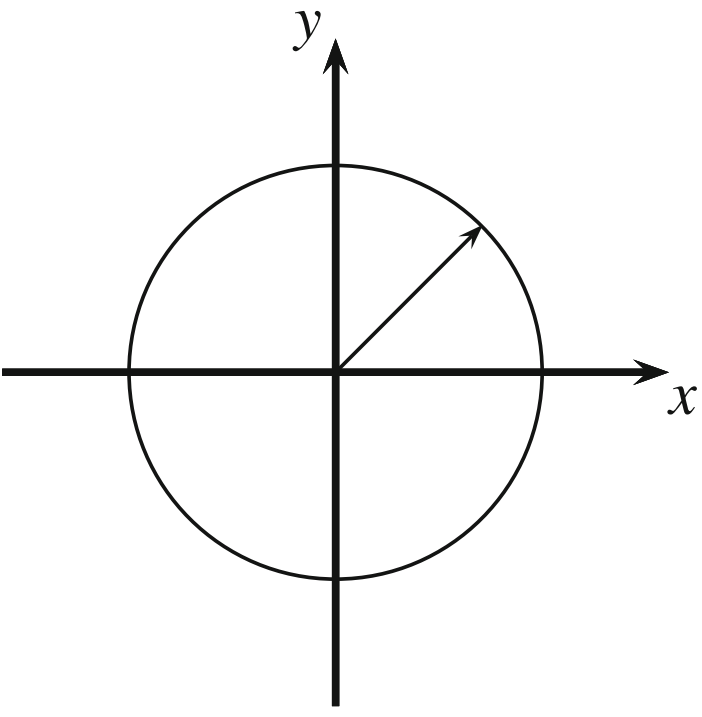
\includegraphics[width=0.3\textwidth]{grafiken/Kreis.PNG}
    \caption[r]{r}
    \label{fig:aufgaben_redesign}
\end{figure}
Die Kreisgleichung kann verallgemeinert werden, indem den Termen $x^2$ und $y^2$ Koeffizienten voran gesetzt werden. Eine solche Gleichung, $ax^2 + by^2 = c$ erzeugt über $\mathbb{R}$ eine Ellipse, wie in Abbildung XY zu sehen.
\begin{figure}[H]
    \centering
    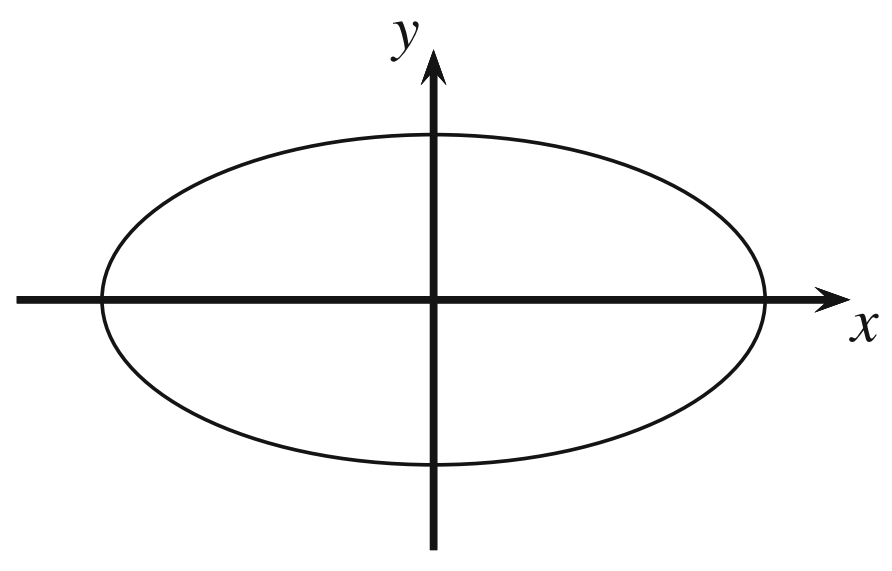
\includegraphics[width=0.3\textwidth]{grafiken/Ellipse.PNG}
    \caption[r]{r}
    \label{fig:aufgaben_redesign}
\end{figure}
Eine elliptische Kurve ist nun eine spezielle Polynomgleichung, der Form $y^2 = x^3 + ax + b$, unter der Bedingung $4a^3 + 27b^3 \neq 0$. Eine solche Gleichung über $\mathbb{R}$ ist in Abbildung XY dargestellt.
\begin{figure}[!h]
    \centering
    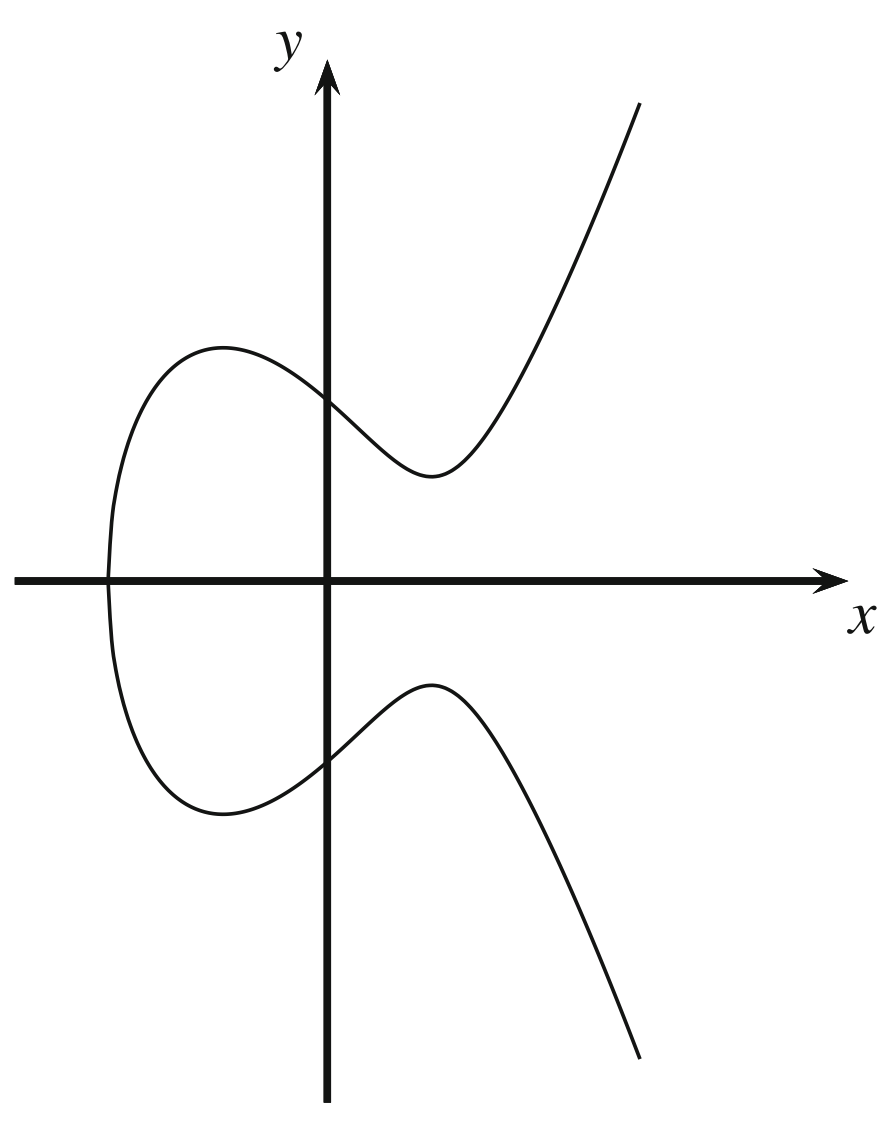
\includegraphics[width=0.3\textwidth]{grafiken/Elliptische_Kurve.PNG}
    \caption[r]{r}
    \label{fig:XXXX}
\end{figure}
Damit elliptische Kurven sinnvoll in der Kryptologie eingesetzt werden können, muss die Polynomgleichung über einem Primkörper betrachtet werden. Das heißt einfach gesprochen, alle Berechnungen werden modulo $p$ durchgeführt.
\paragraph{Definition: Elliptische Kurven über Primkörpern}
Die \textit{elliptische Kurve} über $\mathbb{F_p}$, ist die Menge aller Punkte $(x,y)$ mit $x,y \in \mathbb{F_p}$, welche die folgende Gleichung erfüllen: 
\begin{center}
$y^2 \equiv x^3 + ax + b$ mod $p$, wobei $a,b \in \mathbb{F_p}$
\end{center} 
und die Bedingung  $$4a^3 + 27b^3 \neq 0$$ gelten müssen. Zu der elliptischen Kurve gehört des Weiteren auch der imaginäre \textit{Punkt im Unendlichen} $\mathcal{O}$.\\

Durch die Bedingung XY werden sog. Singularitäten ausgeschlossen. Andernfalls gäbe es Punkte, deren Tangente nicht wohldefiniert ist, was für das Rechnen auf elliptischen Kurven jedoch erforderlich ist.

Nachdem elliptische Kurven nun definiert wurden, stellt sich die Frage, wie diese in der Kryptographie eingesetzt werden können. Wenn wir uns an das in Kapitel XY zurückerinnern, wird für die Konstruktion eines \textbf{DLP}s eine zyklische Gruppe benötigt. Eine eben solche findet sich in der Punktmenge der elliptischen Kurve wieder. Offen bleibt wie die Gruppenoperation definiert ist. Diese muss die in Kapitel XY geforderten Gruppengesetze erfüllen.\\

Als Symbol für die Gruppenoperation wird das Additionszeichen $+$ verwendet. Durch die Gruppenoperation muss aus zwei Punkten $P = (x_1, y_2)$ und $Q= (x_2, y_2)$ der Kurve ein dritter Punkt $R$ auf der Kurve berechnet werden. 
$$P + Q = R$$ $$(x_1, y_1) +  (x_2, y_2) = (x_3, y_3)$$
Am verständlichsten lässt sich diese Operation grafisch zeigen.

Elliptische Kurven über endlichen Körpern können grafisch nicht sinnvoll dargestellt werden. Ihre Form und Arithmetik lassen sich jedoch gut veranschaulichen wenn man sie auf $\mathbb{R}$ abbildet. Im Folgenden betrachten wir eine Elliptische Kurve, dargestellt in einem kartesischen Koordinatensystem, um die Gruppeneigenschaften bezüglich der Punktaddition zu zeigen. Hierbei sind nun zwei Fälle zu unterscheiden.\\

\textbf{Punktaddition $P + Q$:}
Falls $P \neq Q$ erfolgt die geometrische Konstruktion, indem zunächst eine Grade durch die beiden Punkte gelegt wird. Aufgrund der Kurveneigenschaften hat diese immer einen dritten Schnittpunkt mit der Kurve. Dieser wird an der $x$-Achse gespiegelt um den gesuchten Punkt $R$ zu erhalten. Abbildung XY zeigt die beschriebene Konstruktion.

\begin{figure}[H]
    \centering
    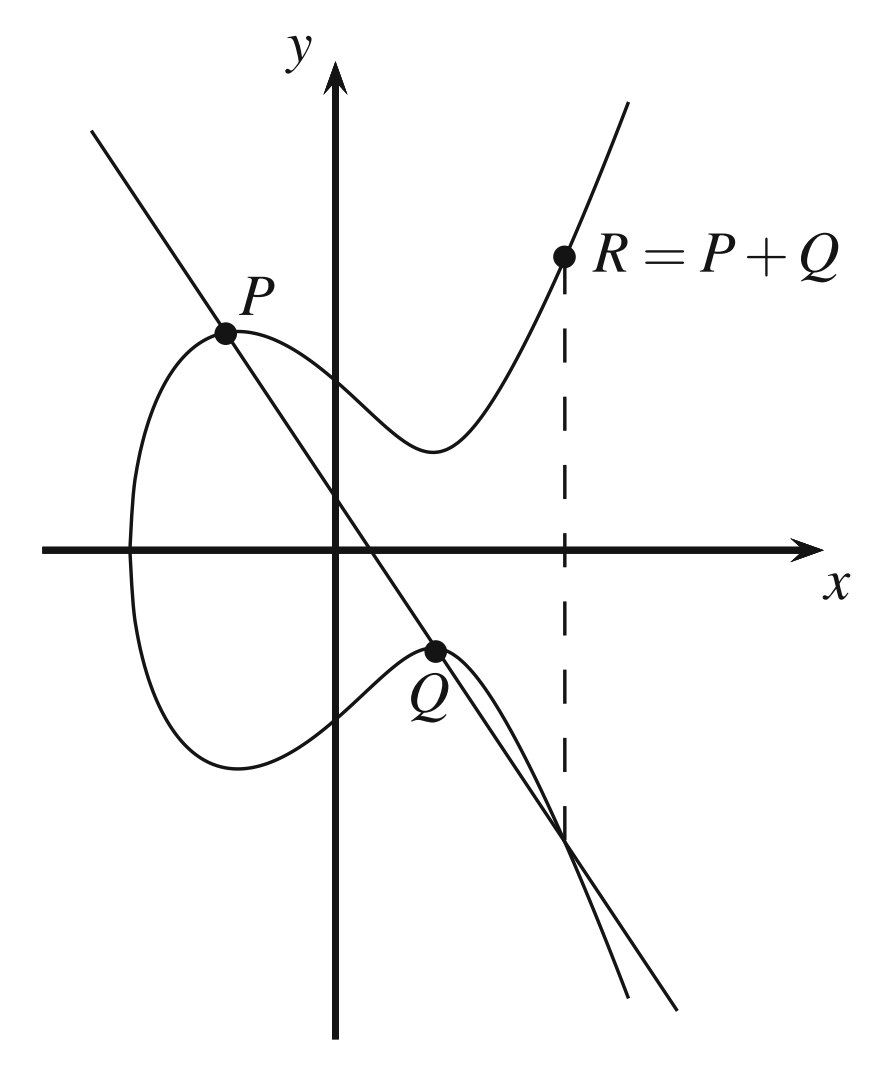
\includegraphics[width=0.3\textwidth]{grafiken/Punktaddition.PNG}
    \caption[Punktaddition]{r}
    \label{fig:Punktaddition}
\end{figure}

\textbf{Punktverdopplung $P + P$:}
Falls P und Q identisch sind erfolgt die geometrische Konstruktion, indem eine Tangente an den Punkt $P$ angelegt wird. Diese liefert wieder einen weiteren Schnittpunkt mit der Kurve, welcher an der $x$-Achse gespiegelt wird um den Punkt $R$ zu erhalten. Anstatt $R = P + Q$ schreibt man in diesem Fall $R = P + P = 2P$   Abbildung XY zeigt die beschriebene Konstruktion. 

\begin{figure}[H]
    \centering
    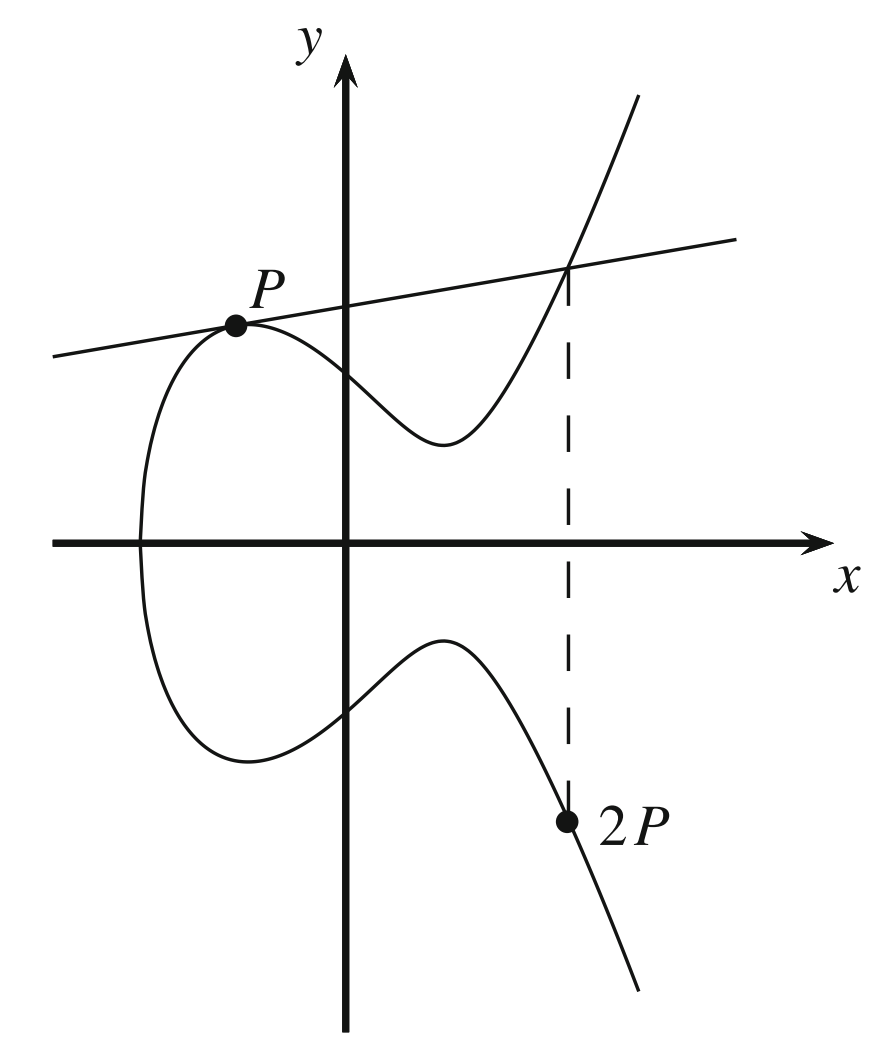
\includegraphics[width=0.3\textwidth]{grafiken/Punktverdopplung.PNG}
    \caption[Punktverdopplung]{r}
    \label{fig:Punktverdopplung}
\end{figure}

Nach dieser grafischen Veranschaulichung sollte es leichter fallen die folgenden Formeln für die Punktaddition bzw. Punktverdopplung nachvollziehen zu können. Die Gruppenoperation existiert in jedem Körper, weshalb die Berechnung von $R$, wie grade gezeigt über den reellen Zahlen $\mathbb{R}$, als auch über einem Primkörper $\mathbb{F_p}$ durchgeführt werden kann.\\

Die Formeln für die Punktaddition und - verdopplung auf elliptischen Kurven können anhand der grade gezeigten Veranschaulichung hergeleitet werden. Das Vorgehen hierbei ist prinzipiell recht simpel.\\ 

Gegeben ist die Gleichung der elliptischen Kurve $y^2 = x^3 +ax + b$ und die Punkte $P = (x_1, y_1)$ und $Q = (x_2, y_2)$. Zunächst ist die Geradengleichung der Sekante durch $P$ und $Q$ zu ermitteln. Eine Grade im Allgemeinen hat die Form $$g: y = sx + m.$$ Der Parameter $s$ ist dabei die Steigung der Geraden und $m$ ist der Schnittpunkt mit der $y$-Achse. Die Steigung $s$ lässt sich wie gewohnt durch Anlegen des Steigungsdreiecks berechnen, also mit der Formel $$s = \frac{y_2 - y_1}{x_2  - x_1}.$$
Zur Bestimmung des Schnittpunkts mit der $y$-Achse kann nun einer der beiden Punkte $P$ oder $Q$ in die Geradengleichung $y = \frac{y_2 - y_1}{x_2  - x_1} * x + m$ eingesetzt werden. Wenn wir $P = (x_1, y_1)$ einsetzen erhalten wir die folgende Gleichung $$y_1 = \frac{y_2 - y_1}{x_2  - x_1} * x_1 + m\text{,}$$ welche nach $m$ aufgelöst folgendermaßen aussieht: $$m = y_1 - \frac{y_2 - y_1}{x_2  - x_1} * x_1$$
Durch Einsetzten aller Parameter in die obige Geradengleichung ergibt sich $$y = \frac{y_2 - y_1}{x_2  - x_1} * x + y_1 - \frac{y_2 - y_1}{x_2  - x_1} * x_1$$ für die gesuchte Gerade $g$ durch die Punkte $P$ und $Q$. Um den dritten Schnittpunkt dieser Geraden $g$ mit der elliptischen Kurve $E$ zu ermitteln, sind beide Kurven gleichzusetzen. Da es für das weitere Vorgehen keine Rolle spielt und es der Übersichtlichkeit dient, werden im Folgenden wieder die Parameter $s$ und $m$ statt eben gezeigten Konkretisierungen verwendet. Es ergibt sich die Gleichung $$(sx+m)^2 = x^3 + ax + b\text{.}$$ Im Normalfall ist das allgemeine Lösen eines solchen kubischen Polynoms nicht trivial. Wir haben hier jedoch den Vorteil, dass zwei der drei Schnittpunkte von $g$ mit $E$ schon bekannt sind. Im Grunde sind wir auf der Suche nach den Nullstellen des kubischen Polynoms, weshalb wir zur Verringerung des Funktionsgrades die Polynomdivision anwenden können, wobei die schon bekannten Nullstellen eben die $x$-Koordinaten der schon bekannten Schnittpunkte sind. Vorher wollen wird die Gleichung durch Umformung auf eine Seite bringen: $$0 =  x^3 - s^2x^2-ax-2smx-m^2+b$$
Die Nullstellen sind $x_1 = x_1$ und $x_2 = x_2$.
Daraus ergibt sich die folgende Polynomdivision:
%$$(x^3 - s^2x^2-ax-2smx-m^2+b) : ((x-x_1)(x-x_2))$$



\textbf{Formel: Punktaddition und -verdopplung auf elliptischen Kurven:}
$$x_3 = s^2 - x_1 - x_2$$
$$y_3 = s(x_1 - x_2) - y_1$$,
wobei

$$s = \begin{cases}
	\frac{y_2 - y_1}{x_2 -x_1} & \text{, falls } P \neq Q \text{ (Punktaddition)}\\
	\frac{3x_1^2 + a}{2y_1} & \text{, falls } P = Q \text{ (Punktverdopplung)}
	\end{cases}
$$

Zur Erfüllung der Gruppeneigenschaften wird außerdem ein neutrales Element $\mathcal{O}$ benötigt. Alle Punkte $P$ der elliptischen Kurve müssen die Eigenschaft $P + \mathcal{O} = P$. Da kein Punkt der elliptischen Kurve diese Eigenschaft erfüllen kann, wird der imaginäre \textit{unendlich ferne Punkt} als neutrales Element $\mathcal{O}$ definiert. Dieser Punkt liefert den dritten \textit{Schnittpunkt} mit der Kurve im Falle, dass ein Punkt $P$ und der bezüglich der $x$-Achse gegenüberliegende Punkt $-P$ addiert werden. Abbildung XY zeigt den Fall grafisch.

Die Existenz eines neutralen Elements ermöglicht die Definition eines Inversen $-P$ für jeden Punkt $P$ auf der Kurve, für welches $P + (-P) = \mathcal{O}$. Wie Abbildung XY  entnommen werden kann, ist für den Punkt $P = (x_p, y_p)$ das Inverse also $-P = (y_p, -y_p)$ zu definieren. In einem Primkörper berechnet sich die negative $y$-Koordinate durch $-y_p = p - y_p$.
 
\section{Punktbestimmung}
Die Arithmetik für Elliptische Kurven wurde bereits besprochen. Nun wird erarbeitet, wie man die Punkte einer elliptischen Kurve bestimmt. Doch was ist ein Punkt einer elliptischen Kurve? Im Foglenden wird erklärt, was ein Punkt auf einer elliptischen Kurve ist und wie diese berehcnet werden können. Die Erklärungen werden anschließend anhand einiger Beispiele näher erläutert. Anschließend wird Python-Code präsentiert, welcher die Punktbestimmung für eine elliptische Kurve mit p > 3 durchführt und die Punkte anschließend in der Konsole ausgibt.

\subsection{Rechnerische Grundlagen}
Viele Mathematiker suchten eine Formel, mit denen sich die Anzahl der Punkte einer elliptischen Kurve schätzen lässt, ohne dass man diese vorher aus- oder berechnen muss. Joseph H. Silverman beweist in seinem Buch einen mathematischen Satz aus der Zahlentheorie, welcher eine allgemeine Aussage über die Anzahl der rationalen Punkte auf einer elliptischen Kurve trifft \cite[vgl.][S. 138]{silverman}. Dieser Satz kann also herangezogen werden, um eine ungefähre Abschätzung über die Anzahl der Punkte auf einer elliptischen Kurve über einem Primkörper p zu treffen. Bei dem mathematischen Satz handelt es sich um die Hasse–Weil–Schranke. Diese wird im allgemeinen dafür benutzt, um die Anzahl der Lösungen der Gleichung und der Bedingungen aber auch für die Einschränkung des Lösungsraums. Die Hasse-Weil-Schranke wird angelehnt an \cite[vgl.][S. 181]{reinholdhuebl} wie folgt beschrieben. Sei k = $\mathbb{F}_p$ ein endlicher Körper und $\overline{E}$ eine elliptische Kurve über k, dann gilt
\begin{center}
$p + 1 - 2 * \sqrt{p} \leq | \overline{E} | \leq p + 1 + 2 * \sqrt{p}$
\end{center} 

Was ist jedoch die Hauptaussage der Hasse-Weil-Schranke? Sie besagt, dass sich bei großen p die Anzahl der Elemente der elliptischen Kurve in der Größenoprdnung von p bewegen. Diese Schranke bildet hierbei eine obere und untere Grenze. Die Anzahl der Punkte bewegt sich also innerhalb dieser Schranke. Dies ist für elliptische Kurven mit kleinem p uninteressant, jedoch wird diese Schranke für elliptische Kurven mit großem gewählten p, was in der Kryptographie gängig ist, relevant.\\


Doch wie lassen sich die Punkte konkret berechnen? Um diese Frage zu beantworten, müssen wir noch einmal die Grundlagen für elliptische Kurven aufgreifen. Wie Reinhold Hübl in seinem Manuskript der Kryptologie \cite[vgl.][S. 157]{reinholdhuebl} erläutert, ist eine elliptische Kurve mit den Charakteristiken char(k) = 0 oder char(k) = 3 eine Kurve, die durch ein Polynom der Form
\begin{center}
$F(X, Y) = Y^{2} - X^{3} - aX - b$
\end{center} 

mit $a, b \in k$ dargestellt ist, für die $4a^3 + 27b^2 \neq 0$  $\in k$ gilt.\\

Stellt man die Gleichung der Funktion nach $y^{2}$ um, dann erhält man folgende Gleichung in zwei Variablen:
\begin{center}
$y^{2} =  x^{3}$ + ax + b  mod(p),
\end{center}

wobei $a, b \in \mathbb{F}_p$. Diese Gleichung ist der Schlüssel für die im Voraus aufgeworfene Frage, was ein Punkt einer elliptischen Kurve ist. Diese sind nämlich alle Punkte (x, y), welche die Gleichung lösen.\\

Um die Punte auf einer Kurve zu berechnen, prüft man zunächst, ob es sich bei der betrachteten Kurve um eine elliptische Kurve mit p > 3 handelt. Dafür arbeitet man mit der Formel  $4a^3 + 27b^2 \neq 0$. Man setzt die Parameter a und b der vermeintlichen elliptischen Kurve ein. Wenn die linke Seite $\neq 0$ ist, dann handelt es sich bei der besagten Kurve tatsächlich um eine elliptische Kurve mit p > 3. Rechnen wir dies nun einmal schematisch durch. Gegeben ist eine Funktion F mit
\begin{center}
$F(X, Y) = Y^{2} - X^{3} + 3X - 3 \in \mathbb{F}_{13}$
\end{center} 

Wie man der Funktion entnehmen kann ist a = - 3 = 10 und b = 3 in $\mathbb{F}_{13}$. Diese setzen wir nun in die Formel ein.
\begin{center}
$4 * 10^3 + 27 * 3^2 = 6 \neq 0$ mod(13)
\end{center} 

Da 6 $\neq$ 0 ist definiert die Funktion eine elliptische Kurve in $\mathbb{F}_{13}$. Die Abbildung \ref{fig:kurve_beispiel_1_punktberechnung} zeigt die Zeichnung der Funktion dieser elliptischen Kurve über den reellen Zahlen im kartesischen Koordinatensystem: 

\begin{figure}[H]
    \centering
    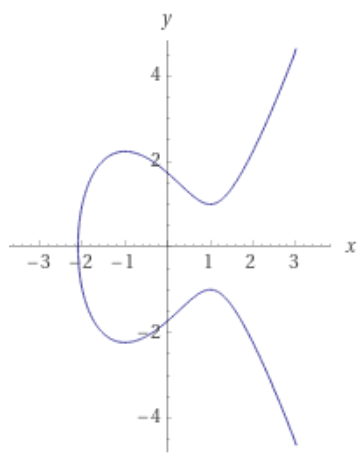
\includegraphics[width=0.5\textwidth]{grafiken/kurve_beispiel_1_punktberechnung.png}
    \caption[Zeichnung der elliptischen Kurve]{Zeichnung der elliptischen Kurve \\ Quelle: Wolframalpha}
    \label{fig:kurve_beispiel_1_punktberechnung}
\end{figure}

Nachdem man allgemein geprüft hat, ob es sich bei der besagten Funktion um eine elliptische Kurve handelt, geht es jetzt um die Findung der Lösungen der umgestellten Gleichung, um alle Punkte zu finden. Dafür gibt es mehrere Möglichkeiten. Die Möglichkeiten haben unterschiedliche Zeit- und Rechenkomplexitäten, wodurch sich die Lösungsmöglichkeiten differenzieren lassen. Je nach Anwendungsfall lohnt sich die Implementierung einer anderen Lösung. Im Folgenden sind zwei Möglichkeiten zur Berechnung aller Punkte auf elliptischen Kurven aufgezählt:

\begin{itemize}
\item Brute-Force
\item Punktaddition und Punktverdopplung
\end{itemize}

Neben dieser zwei gängigen Methoden werden in der Mathematik und in der Kryptografie auch die Barrett-Reduktion und weiterhin auch eine Methode, bei welcher sich die Symmetrie zur x-Achse der elliptischen Kurve zur Berechnung zunutze gemacht wird, genutzt. Um diese soll es jedoch nicht gehen. In den folgenden zwei Unterkapiteln wird die Berechnung der Punkte über Brute-Force sowie über die Punktaddition und -verdopplung erläutert und mittels Beispielen verständlich erklärt.

\subsection{Punktberechnung: Brute-Force-Methode}
Bei der Brute-Force-Methode wird für jeden möglichen Wert x in $\mathbb{F}_p$ von 0 bis p-1 geprüft, ob dieser ein Quadrat in $\mathbb{F}_p$ ist. Wenn bestätigt ist, dass der Wert x ein Quadrat ist, dann setzt man x in die umgestellte Gleichung der elliptischen Kurve in zwei Variablen ein, um die entsprechende y-Koordinate zum besagten x-Wert zu finden. Konnte ein y-Wert zu einem x-Wert gefunden werden, dann ist (x, y) $\in$ E. Beide Werte zusammen ergeben einen Punkt P(x, y) auf der elliptischen Kurve. Die Berechnung der Quadrate erfolgt über XXX

\subsection{Punktberechnung: Punktaddition und -verdopplung}
U

\subsection{Implementierung in Python}
U





































\chapter{Kryptosysteme unter Verwendung elliptischer Kurven}
\section{Diffie-Hellman Key Exchange}
\section{El-Gamal Verschlüsselung}
%3. Implementierung in Python
\chapter{Implementierung in Python}\label{sec:python}
In diesem Kapitel wird die Umsetzung der theoretische Behandelten Konzepte in Python thematisiert. Im Zuge dessen, werden auch die verwendeten Bibliotheken und die Programmiersprache Python kurz thematisiert.\\

Python ist eine höhere Programmiersprache, die in den späten 1980er Jahren entwickelt wurde. Sie wurde entworfen, um die Programmierung einfach, lesbar und zugänglich zu machen. Python ist bekannt für seine klare Syntax und seine Fähigkeit, komplexe Aufgaben mit wenigen Codezeilen zu erledigen. Die Programmiersprache ist zudem sehr flexibel und kann in vielen Bereichen eingesetzt werden, z.B. Webentwicklung, Datenanalyse, wissenschaftliche Programmierung, maschinelles Lernen, Automatisierung, Spieleentwicklung und vieles mehr. Python hat eine große Gemeinschaft von Entwicklern und bietet eine breite Palette von Bibliotheken und Frameworks, die für verschiedene Zwecke verwendet werden können\cite{GuidovanRossum.28.04.2023}. Aufgrund der genannten Eigenschaften wurde für die Umsetzung dieses Projekts Python eingesetzt.\\

Die Bibliothek Numpy wurde verwendet um innerhalb des Programms Berechnungen durchzuführen, welche nicht durch die Standard-Pythonbibliothek bereitgestellt werden. Numpy ist eine Python-Bibliothek, die für numerische Berechnungen und Datenanalyse verwendet wird. Numpy bietet leistungsstarke Funktionen für Arrays und Matrizen sowie für mathematische Funktionen wie lineare Algebra, Fourier-Transformationen und Statistik. Numpy wurde für die Arbeit mit großen Datensätzen und für die schnelle Berechnung von mathematischen Operationen entwickelt. Numpy verwendet C-Code im Hintergrund, um eine höhere Leistung zu erreichen, was sie zu einer beliebten Wahl für wissenschaftliche Berechnungen macht. Numpy wird oft mit anderen Bibliotheken wie Pandas, Scipy und Matplotlib kombiniert, um umfassende Datenaufbereitungs- und Datenanalyse-Tools bereitzustellen \cite{TravisE.Oliphant.o.J.}. In dieser Arbeit wurde nur ein Bruchteil der durch Numpy gebotenen Funktionalitäten genutzt.\\

Zur grafischen Darstellung der elliptischen Kurven wurde die Bibliothek Matbplotlib verwendet. Dies ist eine Python-Bibliothek für die Erstellung von Plots und Diagrammen. Matplotlib ist sehr flexibel und kann für eine Vielzahl von Anwendungen eingesetzt werden, z.B. für die Erstellung von wissenschaftlichen Diagrammen, Finanzdiagrammen, 2D- und 3D-Diagrammen und animierten Diagrammen. Matplotlib ist sehr einfach zu verwenden und bietet eine Vielzahl von Optionen für die Gestaltung von Diagrammen, z.B. Farben, Linienstilen und Textformatierung. Matplotlib wird oft zusammen mit Numpy und anderen Bibliotheken verwendet, um Datenvisualisierung und explorative Datenanalyse zu ermöglichen \cite{JohnD.Hunter.2007}.

Das entwickelte Programm ermöglicht es ermöglicht es elliptische Kurven zu definieren und grafisch darzustellen. Darüber hinaus kann auf Basis einer elliptischen Kurve eine zyklische Gruppe erzeugt werden, welche wiederum die Basis für einen Diffie-Hellman-Key-Exchange darstellt. In der \textit{main.py} werden einige Beispiele für elliptische Kurven mit verschiedener Punkteanzahl gegeben. Zudem werden die implementierten Klassen beispielhaft genutzt um einen DHKE durchzuführen.


\section{Klasse: ellipticCurveInFp}
Die Klasse \textit{ellipticCurveInFp} ermöglicht es eine elliptische Kurve der Form $$y^2 = x^3 + ax + b \in \mathbb{F}_p$$ zu definieren. Im Zuge dessen werden verschiedene Methoden bereitgestellt.

\subsection{Methode: get\_all\_points\_on\_curve()}
Mittels des in Kapitel \ref{sec:brute_force} vorgestellte Verfahrens ermittelt diese Funktion alle auf der elliptischen Kurve befindlichen Punkte.

\vspace{\baselineskip}
\begin{lstlisting}[caption={Methode: get\_all\_points\_on\_curve()}, captionpos=b]
def get_all_points_on_curve(self):
    if not self.is_elliptic_curve_correct():
        return False
    # Berechnen der Quadrate und zugehoerige Wurzeln in F_p
    squares_with_roots = supportAlgos.get_squares_with_roots(range(self.p))
    # Liste mit Quadraten erstellen
    squares = []
    for tupel in squares_with_roots:
        if tupel[0] not in squares:
            squares.append(tupel[0])
    # Pruefe fuer jedes x in F_p, ob es eingesetzt ein Quadrat ergibt
    x_values = []
    for x in range(self.p):
        if (x ** 3 + self.a * x + self.b) % self.p in squares:
            x_values.append(x)
    # Ermitteln der Punkte auf der Kruve
    points = []
    for x in x_values:
        y_quad = (x ** 3 + self.a * x + self.b) % self.p
        for tupel in squares_with_roots:
            if y_quad == tupel[0]:
                points.append((x, tupel[1]))
    # Neutrales Element hinzufuegen
    points.append(("N", "N"))
    return points
\end{lstlisting}
\vspace{\baselineskip}

Zunächst wird geprüft, ob die elliptische Kurve korrekt definiert ist. Durch die Funktion \textit{get\_squares\_with\_roots()} wird zu jeder Zahl von $0$ bis $p-1$ das Quadrat in $\mathbb{F}_p$ berechnet. Die errechneten Quadrate werden in einer Liste gespeichert. Anschließend wird jedes $x > p$ in die Gleichung der elliptischen Kurve eingesetzt um zu prüfen ob das Ergebnis einem der errechneten Quadrate entspricht. Jene $x$-Werte auf die das zutrifft, werden in einer Liste gespeichert. Anschließend werden für jeden dieser $x$-Werte die zugehörigen $y$-Werte ermittelt und die Kombination als Punkte in einer Liste gespeichert. Im letzten Schritt wird der Liste der unendlich ferne Punkt hinzugefügt und die List zurückgegeben.
\subsection{Methode: is\_elliptic\_curve\_correct()}
Diese Methode prüft alle Eigenschaften, die zur Definition einer Elliptischen Kurve erforderlich sind und gibt entsprechend \textit{True} oder \textit{False} zurück.

\vspace{\baselineskip}
\begin{lstlisting}[caption={Methode: is\_elliptic\_curve\_correct()}, captionpos=b]
def is_elliptic_curve_correct(self):
	# p muss eine Primzahl sein
	if not is_prime(self.p):
		return False
	# p muss groesser als 3 sein
    if self.p <= 3:
        return False
	# 4a^3 + 27b^2 darf nicht durch p teilbar sein bzw. nicht Null sein in F_p
	if (4 * (self.a ** 3) + 27 * (self.b ** 2)) % self.p == 0:
		return False
	# Die Kurve ist korrekt
    return True
\end{lstlisting}
\vspace{\baselineskip}
Im ersten Schritt wird überprüft ob es sich beim Parameter $p$ um eine Primzahl handelt, da $\mathbb{F}_p$ ein Primkörper sein muss. Im zweiten Schritt wird geprüft ob $p > 3$, da der Arithmetik auf Kurven mit $p <= 3$ andere Formeln zur Punktaddition zu Grunde liegen, mit welchen hier nicht Umgegangen werden kann. Als letzten Schritt wird die Bedingung $$4x^3 + 27x^2 \neq 0 \in \mathbb{F}_p$$ geprüft. Diese muss, wie in Kapitel \ref{sec:elliptische_kurve} erwähnt, gelten sein um Singularitäten auszuschließen.

\subsection{Methode: is\_point\_on\_curve()}
Die Methode überprüft ob ein gegebener Punkt auf der definierten elliptischen Kurve liegt.

\vspace{\baselineskip}
\begin{lstlisting}[caption={Methode: is\_point\_on\_curve()}, captionpos=b]
def is_point_on_curve(self, P):
	x, y = P
    # y^2 = x^3 + ax + b muss erfuellt sein in F_p
    return (y ** 2 - x ** 3 - self.a * x - self.b) % self.p == 0
\end{lstlisting}
\vspace{\baselineskip}
Dazu wird geprüft ob nach Einsetzten des gegebenen Punktes die Kurvengleichung $$y^2 = x^3 + ax + b \in \mathbb{F}_p$$ erfüllt ist. Entsprechend wird \textit{True} oder \textit{False} zurückgegeben.

\subsection{Methode: add()}
Die \textit{add()} Methode dient dazu zwei Punkte auf der elliptischen Kurve zu addieren. Zur Abbildung des unendlich fernen Punkts bzw. des neutralen Elements wurde die Notation $(N,N)$ gewählt. Aufgrund der Ähnlichkeit zu $(0,0)$, wurde nicht von $(O,O)$ Gebrauch gemacht, was wegen der Bezeichnung des neutralen Elements $\mathcal{O}$ naheliegend wäre. 

\vspace{\baselineskip}
\begin{lstlisting}[caption={Methode: add()}, captionpos=b]
def add(self, P, Q):
    x1, y1 = P
    x2, y2 = Q
    # Addition des neutralen Elements mit sich selbst ergibt das neutrale Element
    if x1 == "N" and x2 == "N":
        R = ("N", "N")
        return R
    # Addition eines Punktes und des neutralen Elements ergibt den Punkt
    elif x1 == "N":
        R = (x2, y2)
        return R
    elif x2 == "N":
        R = (x1, y1)
        return R
    # Addition inverser Punkte ergibt neutrales Element
    elif x1 == x2 and y1 != y2:
        R = ("N", "N")
        return R

        # Addition nach bekannten Formeln
        if x1 == x2 and y1 == y2:
            # Punkt ist Nullstelle --> Tangente ist parallel zur y-Achse --> ergibt neutrales Element
            if y1 == 0:
                R = ("N", "N")
                return R
            # Punktaddition mit sich selbst
            s = (3 * x1 ** 2 + self.a) * supportAlgos.inverse_mod(2 * y1, self.p) % self.p
        else:
            # Punktaddition von unterschiedlichen Punkten
            s = (y2 - y1) * supportAlgos.inverse_mod(x2 - x1, self.p) % self.p
        x3 = (s ** 2 - x1 - x2) % self.p
        y3 = (s * (x1 - x3) - y1) % self.p
        R = (x3, y3)
        return R
\end{lstlisting}
\vspace{\baselineskip}
Zunächst werden alle Sonderfälle behandelt:
\begin{itemize}
\item $\mathcal{O} + \mathcal{O} = \mathcal{O}$
\item $P + \mathcal{O} = \mathcal{O} + P = P$
\item $P + -(P) = \mathcal{O}$
\item Falls $P = (x_P, 0)$, dann gilt $P + P = \mathcal{O}$
\end{itemize}
Nach Behandlung dieser Sonderfälle erfolgt die Berechnung von $R = (x_3, y_3)$ gemäß den in Kapitel \ref{sec:Arithmetik} hergeleiteten Formeln:
$$x_3 = s^2 - x_1 - x_2$$
$$y_3 = s(x_1 - x_3) - y_1$$,
wobei

$$s = \begin{cases}
	\frac{y_2 - y_1}{x_2 -x_1} & \text{, falls } P \neq Q \text{ (Punktaddition)}\\
	\frac{3x_1^2 + a}{2y_1} & \text{, falls } P = Q \text{ (Punktverdopplung)}
	\end{cases}
$$
\vspace{\baselineskip}

\section{Klasse: CyclicGroup}
Diese Klasse bietet Funktionalitäten bezüglich der Gruppeneigenschaften elliptischer Kurven. Ein Objekt der Klasse \textit{EllipticCurveInFp} muss im Konstruktor übergeben werden. \textit{CyclicGroup} stellt Methoden zur Addition und Skalar-Multiplikation, als auch jene zur Bestimmung der Gruppen- und Elementordnung etc. zur Verfügung.
\subsection{Methode: add\_elements()}
Diese Methode stellt die Funktionalität bereit, zwei Gruppenelemente zu addieren und das Ergebnis zurückzugeben. Dazu wird intern die \textit{add()} Methode der \textit{EllipticCurveInFp}-Klasse genutzt.
\vspace{\baselineskip}
\begin{lstlisting}[caption={Methode: add\_elements()}, captionpos=b]
def add_elements(self, A, B):
	C = self.elliptic_curve.add(A, B)
    return C
\end{lstlisting}
\vspace{\baselineskip}

\subsection{Methode: scalar\_dot\_element}
Die Methode \textit{scalar\_dot\_element()} ermöglicht es, einen Punkt auf der Kurve mit einem Skalar zu multiplizieren. Dabei wird der in Kapitel \ref{sec:DLPüberEC} erläuterte Doubble-And-Add-Algorithmus verwendet.

\vspace{\baselineskip}
\begin{lstlisting}[caption={Methode: scalar\_dot\_element()}, captionpos=b]
def scalar_dot_element(self, scalar, element):
    binary = bin(scalar)
    binary = binary[3:]
    # double and add algorithm
    current_element = element
    for digit in binary:
        # double
        current_element = self.add_elements(current_element, current_element)
        if digit == "1":
            # add
            current_element = self.add_elements(current_element, element)
    return current_element
\end{lstlisting}
\vspace{\baselineskip}
Nach Durchlauf des Algorithmus wird der zuletzt berechnete Punkt zurückgegeben.

\subsection{Methode: get\_sub\_group\_elements()}
Unter Anwendung des Wissens aus dem Kapitel zu Untergruppen zyklischer Gruppen \ref{sec:untergruppen} findet diese Methode alle Element der durch einen Punkt bzw. Gruppenelement generierten Untergruppe. Dazu wird der Punkt so lange zu sich selbst addiert, bis das neutrale Element erreicht wird. Alle dabei berechneten Punkte gehören zur durch den gegebenen Punkt erzeugten Untergruppe.

\vspace{\baselineskip}
\begin{lstlisting}[caption={Methode: get\_sub\_group\_elements()}, captionpos=b]
def get_sub_group_elements(self, primitive_element):
    current_element = primitive_element
    sub_group_elements = []
    while True:
        sub_group_elements.append(current_element)
        current_element = self.add_elements(current_element, primitive_element)
        if current_element == primitive_element:
            break
    return sub_group_elements
\end{lstlisting}
\vspace{\baselineskip}

In jedem Schleifendurchlauf wird der errechnete Punkt einer List hinzugefügt, welche nach Erreichen des neutralen Elements zurückgegeben wird.

\subsection{Methode: get\_element\_order()}
Diese Methode gibt die Ordnung eines gegebenen Gruppenelements wieder. Dazu wird mittels der Methode \textit{get\_sub\_group\_elements()} die durch das Element erzeugte Untergruppe ermittelt. Die Anzahl der ermittelten Elemente entspricht der Ordnung des Elements.

\vspace{\baselineskip}
\begin{lstlisting}[caption={Methode: get\_element\_order()}, captionpos=b]
def get_element_order(self, element):
	sub_group_elements = self.get_sub_group_elements(element)
	order = len(sub_group_elements)
    return order
\end{lstlisting}
\vspace{\baselineskip}

\subsection{Methode: get\_group\_order()}
Mittels dieser Methode kann die Gruppenordnung bestimmt werden. Diese entspricht der Anzahl der Punkte auf der elliptischen Kurve, weshalb intern auf die Methode \textit{get\_all\_points\_on\_curve()} der Klasse \textit{EllipticCurveInFp} zurückgegriffen wird. Jene liefert alle Punkte auf der Kurve, deren Anzahl anschließend ermittelt und zurückgegeben wird.

\vspace{\baselineskip}
\begin{lstlisting}[caption={Methode: get\_group\_order()}, captionpos=b]
def get_group_order(self):
    group_elements = self.elliptic_curve.get_all_points_on_curve()
    group_order = len(group_elements)
    return group_order
\end{lstlisting}
\vspace{\baselineskip}

\subsection{Methode: get\_group\_elements()}
Durch diese Methode werden alle Gruppenelemente zurückgegeben. Diese entsprechen den Punkten auf der elliptischen Kurve, weshalb wieder die \textit{get\_all\_points\_on\_curve()}-Methode der Klasse \textit{EllipticCurveInFp} genutzt wird.

\vspace{\baselineskip}
\begin{lstlisting}[caption={Methode: get\_group\_elements()}, captionpos=b]
def get_group_elements(self):
	return self.elliptic_curve.get_all_points_on_curve()
\end{lstlisting}
\vspace{\baselineskip}
  
\subsection{Methode: get\_all\_sub\_groups()}
Diese Methode gibt alle Untergruppen der zyklischen Gruppe in einer Liste wieder. Dazu wird der Satz \textit{Konstruktion einer zyklischen Untergruppe} aus Kapitel \ref{sec:untergruppen} angewandt. Dieser besagt im Kern, dass nur die Gruppenkardinalität sowie ein primitives Element benötigt wird, um alle Untergruppen zu ermitteln.
\vspace{\baselineskip}
\begin{lstlisting}[caption={Methode: get\_all\_sub\_groups()}, captionpos=b]
def get_all_sub_groups(self):
    sub_groups = []
    sub_group_generators = []
    divisors = []
    order = self.get_group_order()
    primitive_elements = self.get_primitive_elements()
    # Finden von echten Teilern der Gruppenordnung
    for number in range(int(order/2 + 1)):
        if order % number == 0:
            divisors.append(number)
    # Berechnen der Untergruppen-Generatoren
    for div in divisors:
        sub_group_generators.append(self.scalar_dot_element((order/div), primitive_elements[0]))
    # Berechnen der Untergruppen
    for gen in sub_group_generators:
        sub_groups.append(self.get_sub_group_elements(gen))
    return sub_groups
\end{lstlisting}
\vspace{\baselineskip}
Zunächst werden unter Verwendung der Methoden \textit{get\_group\_order()} und \textit{get\_primitive\_elements()} die Gruppenordnung und die primitiven Elemente ermittelt. Im Grunde wird aber nur ein primitives Element benötigt. Im folgenden Schritt werden die echten Teiler der Gruppenordnung identifiziert und gespeichert. Um die Generatoren der Untergruppen zu finden, wird anschließend für jeden echten Teiler das primitive Element mit  $\frac{Gruppenordnung}{echter Teiler}$ multipliziert. Nach Erhalt der Generatoren, wir mittels der Methode \textit{get\_sub\_group\_elements} für jeden Generator die erzeugte Untergruppe berechnet und diese in einer List gespeichert, welche schlussendlich zurückgegeben wird. 
\subsection{Methode: get\_primitive\_elements()}
Primitive Elemente zeichnen sich dadurch aus, dass ihre Ordnung der Gruppenordnung entspricht, sie also bei Addition zu sich selbst die gesamte Gruppe generieren. Die Methode \textit{get\_primitive\_elements()} prüft für jedes Element der Gruppe dessen Ordnung und gibt eine Liste jener Elemente zurück deren Ordnung der Gruppenordnung entspricht.

\vspace{\baselineskip}
\begin{lstlisting}[caption={Methode: get\_primitive\_elements()}, captionpos=b]
def get_primitive_elements(self):
    elements = self.get_group_elements()
    group_order = self.get_group_order()
    primitive_elements = []
    for element in elements:
        if self.get_element_order(element) == group_order:
            primitive_elements.append(element)
    return primitive_elements
\end{lstlisting}
\vspace{\baselineskip}

\section{Klasse: DHKE}
Die Klasse \textit{DHKE} nutz die Methoden der Klasse \textit{CyclicGroup} um die Funktionalität für einen Elliptic-Curve-Diffi-Hellman-Key-Exchange durchzuführen. Die Implementierung könnte genauso gut für einen klassischen DHKE genutzt werden, was im Grunde von der Übergebenen zyklischen Gruppe abhängt, daher der Name DHKE anstatt ECDHKE. Wie schon a ngedeutet wird der Klasse im Konstruktor die zugrundeliegende zyklische Gruppe übergeben.
\subsection{Methode: gen\_key\_pair()}
Basierend auf einem gegebenen Generator erzeugt die Methode ein Schlüsselpaar bestehend aus einem zufälligen privaten Schlüssel und einem daraus berechneten öffentlichen Schlüssel.
\vspace{\baselineskip}
\begin{lstlisting}[caption={Methode: get\_primitive\_elements()}, captionpos=b]
def gen_key_pair(self, start_element):
    group_order = self.cyclic_group.get_element_order(start_element)
    # k_priv = random.randrange(int(np.sqrt(10000000000000000000)), 10000000000000000000)
    k_priv = np.random.randint(np.sqrt(group_order), group_order)
    # kPub = kPriv * start_point
    k_pub = self.cyclic_group.scalar_dot_element(k_priv, start_element)
    self.k_priv = k_priv
    self.k_pub = k_pub
    return k_priv, k_pub
\end{lstlisting}
\vspace{\baselineskip}

Im ersten Schritt wird mittels der Methode \textit{get\_element\_order()} der Klasse \textit{CyclicGroup} die Ordnung des Generators $g$ ermittelt. Anschließend wird ein zufälliger privater Schlüssel $k_{priv} \in \{\sqrt{ord(g)},..., ord(g)\}$ erzeugt. Dieser private Schlüssel wird nun unter Verwendung der Methode \textit{scalar\_dot\_element()} aus der Klasse \textit{CyclicGroup} mit dem gegebenen Generator multipliziert um den öffentlichen Schlüssel $k_{pub}$ zu erzeugen. Beide Schlüssel werden in Objektattributen gespeichert um sie weiteren verwenden zu können und anschließend zurückgegeben.

\subsection{Methode: calc\_common\_key()}
Nach Erhalt des öffentlichen Schlüssel des Kommunikationspartners ermöglicht es diese Methode den gemeinsamen geheimen Schlüssel zu berechnen.

\vspace{\baselineskip}
\begin{lstlisting}[caption={Methode: calc\_common\_key()}, captionpos=b]
def calc_common_key(self, k_pub):
	common_key = self.cyclic_group.scalar_dot_element(self.k_priv, k_pub)
	return common_key
\end{lstlisting}
\vspace{\baselineskip}
Dies geschieht durch die Multiplikation des eigenen privaten Schlüssel mit dem gegebenen öffentlichen Schlüssel des Kommunikationspartners. Der berechnete Schlüssel wird folgend zurückgegeben.

\section{Support Algorithmen}
Neben den oben gezeigten Klassen wurde ein Modul mit verschiedenen Algorithmen entwickelt, welche von den anderen Klassen verwendet werden.

\subsection{Funktion: is\_prime()}
Die \textit{is\_prime}-Funktion ermöglicht es festzustellen ob eine gegebene Zahl eine Primzahl ist. Im Falle einer Primzahl wird \textit{True}, ansonsten \textit{False} zurückgegeben.
\vspace{\baselineskip}
\begin{lstlisting}[caption={Funktion: is\_prime()}, captionpos=b]
def is_prime(n):
    if n <= 1:
        return False
    for i in range(2, int(math.sqrt(n)) + 1):
        if n % i == 0:
            return False
    return True
\end{lstlisting}
\vspace{\baselineskip}
Zunächst wird geprüft ob die gegebene Zahl $n$ kleiner oder gleich 1, da es in dem Fall sicher keine Primzahl ist. Danach wird für jede Zahl von $2$ bis $\sqrt{n}$ geprüft ob sie ein Teiler von $n$ ist. Falls ein Teiler gefunden wird, ist $n$ keine Primzahl, falls nicht, ist $n$ eine Primzahl.

\subsection{Funktion: extended\_euclidean\_algorithm()}
Diese Funktion ist eine rekursive Implementierung des erweiterten euklidischen Algorithmus. Dieser liefert neben dem $GGT$ der beiden Inputparameter $a$ und $b$ auch die Koeffizienten der Gleichung $$ax + by == GGT$$. In der Praxis wird die häufig eingesetzt um das multiplikative Inverse einer Zahl in einem endlichen Körper zu berechnen.
\vspace{\baselineskip}
\begin{lstlisting}[caption={Funktion: extended\_euclidean\_algorithm()}, captionpos=b]
def extended_euclidean_algorithm(a, b):
    if a == 0:
        return b, 0, 1
    else:
        gcd, x, y = extended_euclidean_algorithm(b % a, a)
        return gcd, y - (b // a) * x, x
\end{lstlisting}
\vspace{\baselineskip}

\subsection{Funktion: inverse\_mod()}
Mittels des erweiterten euklidischen Algorithmus berechnet diese Funktion das multiplikative Inverse einer Zahl $a$ modulo $m$.

\vspace{\baselineskip}
\begin{lstlisting}[caption={Funktion: inverse\_mod()}, captionpos=b]
def inverse_mod2(a, m):
    gcd, x, y = extended_euclidean_algorithm(a, m)
    if gcd != 1:
        return None
    else:
        return x % m
\end{lstlisting}
\vspace{\baselineskip}

Im Fall, das der $GGT$ von $a$ und $m$ ungleich 1 ist, was gleichbedeutend damit ist, dass kein Inverses existiert, wird \textit{None} zurückgegeben, ansonsten das  multiplikative Inverse.

\subsection{Funktion: get\_squares\_with\_roots()}
Diese Funktion gibt bei einer gegebenen Liste von Zahlen zu jeder Zahl das Quadrat modulo der Anzahl der Zahlen wieder. Die Funktion wird im Zuge der Punktbestimmung verwendet.
\vspace{\baselineskip}
\begin{lstlisting}[caption={Funktion: get\_squares\_with\_roots()}, captionpos=b]
def get_squares_with_roots(candidate_list):
    squares_with_roots = []
    for x in candidate_list:
        square = (x ** 2) % len(candidate_list)
        squares_with_roots.append((square, x))

    return squares_with_roots
\end{lstlisting}
\vspace{\baselineskip}
Für jede Zahl in der Liste wird das Quadrat in $\mathbb{F}_p$ berechnet und anschließend werden alle Tupel in der Form $(Quadrat, Wurzel)$ zurückgegeben.

\subsection{Funktion: eratosthenes()}
Mit Hilfe des Siebes des Eratosthenes können alle Primzahlen bis zu einem Parameter \textit{limit} berechnet, zu der Liste \textit{primes} hinzugefügt und auch angezeigt werden. Es wird eine Liste mit allen Zahlen von 2 bis \textit{limit} + 1 erstellt. In einer folgenden Schleife wird durch jede Zahl in der Liste durchiteriert und es wird geprüft, ob sie durch eine Zahl in der Liste teilbar ist. Wenn ja, dann wird die Zahl aus der ersten Liste entfernt. Am Ende bleiben alle Zahlen in der Liste \textit{primes}, welche keine Teiler haben. 

\vspace{\baselineskip}
\begin{lstlisting}[caption={Funktion: eratosthenes(limit)}, captionpos=b]
def eratosthenes(limit):
    primes = []
    for number in range(2, limit + 1):
        primes.append(number)
    # print(primes)

    for prime in primes:
        for number in primes[primes.index(prime) + 1:]:
            if number % prime == 0:
                primes.remove(number)

    print(primes)
    return primes
\end{lstlisting}
\vspace{\baselineskip}

Für das Durchlaufen der Zahlen bis zum eingegebenen Limit werden mehrere Schleifen benötigt. 

\newpage
\end{onehalfspacing}
\printbibliography
\end{document}